\documentclass[11pt]{article}
\usepackage[utf8]{inputenc}
\usepackage[T1]{fontenc}
\usepackage{hyperref}
\usepackage[authoryear]{natbib}
\usepackage{textcomp}
\usepackage{subcaption}
\usepackage{graphicx}
\usepackage{fancybox}
\usepackage{xcolor}
\usepackage{makeidx}
\usepackage{float}
\usepackage{amsmath,amssymb}
\usepackage{eurosym}

\usepackage{enumitem}
\PassOptionsToPackage{normalem}{ulem}
\usepackage{ulem}
\hypersetup{citecolor=blue,colorlinks=true}

\usepackage{multicol}
\usepackage[toc,page]{appendix}
\usepackage{array,multirow,makecell}
\usepackage[modulo]{lineno}
\renewcommand{\arraystretch}{0.73}
\setcellgapes{1pt}
\makegapedcells
\renewcommand*\thetable{\Roman{table}}
\renewcommand*\thefigure{\Roman{figure}}
\renewcommand{\thetable}{\Alph{section}.\arabic{table}}
\renewcommand{\thefigure}{\Alph{section}.\arabic{figure}}
\usepackage{chngcntr}
\counterwithin{figure}{section}
\counterwithin{table}{section}
\renewcommand{\floatpagefraction}{1}
%\renewcommand{\footnotelayout}{\setstretch{0.5}}
\newcolumntype{R}[1]{>{\raggedleft\arraybackslash }b{#1}}
\newcolumntype{L}[1]{>{\raggedright\arraybackslash }b{#1}}
\newcolumntype{C}[1]{>{\centering\arraybackslash }b{#1}}
\usepackage[left=2.5cm,right=2.5cm,top=2.5cm,bottom=2.5cm]{geometry}
\linespread{1.5}
\date{}
\hypersetup{citecolor=blue,colorlinks=true}
%\setlength{\parindent}{1pt}

\title{Supplementary material to \textit{French Attitudes over Climate Change, the Carbon Tax and Other Climate Policies}}
\author{Thomas Douenne and Adrien Fabre\footnote{Paris School of Economics.  thomas.douenne@psemail.eu ; adrien.fabre@psemail.eu}} 
%\date{$\textnormal{\today}$}

\linespread{1}\selectfont

\begin{document}
\maketitle
%\sloppy


  
%\textit{This online appendix contains supplementary material to the paper titled ``French Attitudes over Climate Change and Climate Policies''. In a first section we detail the survey.}



\setcounter{tocdepth}{1}
\tableofcontents
%%TC:endignore

%\vfill\eject 
%\linenumbers



\section{Additional results on attitudes over climate change}
    

      \subsection{Perceptions\label{subsec:opinions}
      }

The looming threat of CC already seems to impact people's behavior. Indeed, 20\% say the CC ``has had or will have an influence in their decision to have a child''. Among them, 37\% justify it ``because each additional human aggravates climate change'', and 86\% because they ``don't want [their] child to live in a devastated world''. This result echoes a survey from \citet{ademe_representations_2018} which shows that 63\% of French people think that ``living conditions will be extremely harsh'' in France in 50 years and that 57\% do not think CC ``will be limited to acceptable levels by the end of the century''. Such concern is not limited to France, as \citet{funk_politics_2016} document that 75\% of American are concerned by CC. Nor is it recent, as Eurobarometer surveys cited by \citet{whitmarsh_2_2018} found that more than three-quarters of respondents were already worried about climate change in 1988, rising to almost nine in ten by 1992.

Despite --- or perhaps due to --- widespread hopelessness, 34\% almost never talk about CC (Figure \ref{fig:talks}). 27\% talk about CC several times per month, which can give a sense of the share of people who regularly engage in long-term thinking. The relatively low amount of discussion around an issue largely perceived as a serious threat may be understood as a way to flee from one's moral duty and to protect one's lifestyle. Indeed, as a recent literature has shown, people tend to discard information perceived as bad news and display what \citet{sharot_et_al_2011} call ``unrealistic optimism in front of reality''. \citet{whitmarsh_2_2018} relate another strategy of avoidance: the general tendency to discount one’s own contribution to causing CC and identify causes of CC primarily with other people or countries. %(Lorenzoni & Pidgeon, 2006; Whitmarsh, 2009)


\begin{figure}[!htbp] % !htbp
\centering
\includegraphics[width=.6\columnwidth]{CC_talks_nolegend.eps}
\caption{Frequency at which respondents talk about climate change.}
\label{fig:talks}
\end{figure}

\begin{figure}
    \centering

    \begin{minipage}{0.49\textwidth}
        \centering
        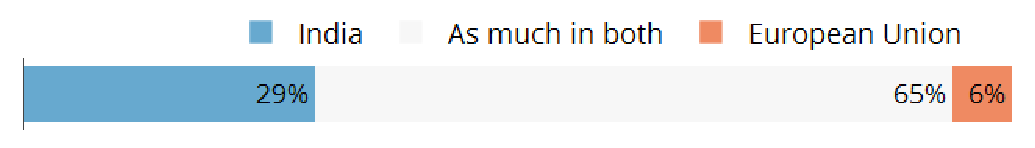
\includegraphics[width=0.99\textwidth]{CC_region_nolegend.eps} % second figure itself
        \caption{Perceived region where climate change impacts will be the most serious.} \label{fig:region}
    \end{minipage} \hfill
        \begin{minipage}{0.49\textwidth}
        \centering
        \includegraphics[width=0.99\textwidth]{CC_generation_min_nolegend_trim.eps} % first figure itself
        \caption{Perceived date of birth of first generation severely affected by CC.} \label{fig:generation}
    \end{minipage}
\end{figure}


One can wonder if this blindness to the causes is mirrored by a sentiment that oneself will not be impacted. This does not seem to be the case on a spatial dimension. Indeed, Figure \ref{fig:region} shows that although five times more people (correctly\footnote{See e.g. vulnerability indexes \citep{climate_vulnerable_forum_climate_2012,guillaumont_measuring_2015,closset_physical_2018}.}) believe that India will face more serious climate impacts than the European Union, 65\% still think that both regions will face as much damage. Yet, the evidence is mild regarding the time dimension, as 45\% of American think that ``global warming will pose a serious threat to [them] or [their] way of life in [their] lifetime'' \href{https://news.gallup.com/poll/1615/environment.aspx}{(Gallup, 2019)} while 62\% of French people think that the first generation seriously affected by CC is yet to be born (Figure \ref{fig:generation}).\footnote{We assume here that both countries are comparable.} 
Interestingly, a delay of one generation as the first (perceived as) affected by CC is significantly associated with a lower knowledge index by 0.1 standard deviation. This finding may indicate that learning is partly motivated by perceived personal prejudice.



    \subsection{The Reaction Needed\label{subsec:reaction}}

\citet{kallbekken_aasen_2010} report that ``a poll of 22,000 respondents from 21 countries found that 83\% say it will be necessary to make lifestyle and behavioural changes to reduce emissions of greenhouse gases (Globescan and PIPA, 2007).'' Other French representative surveys find similar results for the reaction needed and indicate which efforts people are most ready to make. \href{http://www.bva.fr/data/sondage/sondage_fiche/1063/fichier_bva_actuc0a25.pdf }{BVA (2011)} indicates that, to save energy, 76\% plan to ``change their consumption habits'' and 61\% plan works in their accomodation. In the U.S., 52\% already think they ``do a good job at protecting the environment'' \href{https://news.gallup.com/poll/1615/environment.aspx}{Gallup (2019)}. However, \citet{ademe_representations_2018} shows that the efforts people are making or could easily make are also the least efficient to reduce GhG emissions: most people cite waste sorting (89\%) or buying seasonal vegetables (87\%), but fewer mention walking or cycling (55\%) or using public transport (49\%) instead of driving. 

% (\citealt{ademe_representations_2018}, \href{http://www.datapressepremium.com/rmdiff/2008572/Etude-OpinionWay-pour-PrimesEnergie.fr.pdf}{OpinionWay 2019})

% autre reactions: ADEME  Si des changements importants s’avèrent nécessaires dans nos modes de vie, à quelles conditions les accepteriez-vous ? 45\% qu'ils soient partagés de façon juste entre tous les membres de notre société, 11\% Qu'ils restent dans des proportions modérées, je ne suis pas prêt à accepter des changements radicaux dans mon mode de vie, 15\% accepterai dans tous cas / fait déjà: moins viande 45\%, vélo/pied plutôt que voiture 35\%, consommer moins 47\% ; peut pas-difficilement moins voiture : 16-19\% (plus optimiste qu'IFOP 11, cf. aussi OpinionWay), 8-15 viande
% OpinionWay: aliments de saison, local, "réduire conso, recycler, échanger", plus de marche et vélo sont les efforts personnellement prêts à être consentits par une majorité, privilégier transports en commun 34\%, le train ou le bus à l'avion pour longues distances 21\%, "consommer moins de viande, d'oeufs et de produits laitiers" 31\%
% BVA 58\% pensent qu'ils consommeront moins d'énergie dans 10 ans en 2011, 61\% veulent faire réaliser des travaux d'économie d'énergie et 76\% changer leurs habitudes de consommation, 48\% pensent utiliser le solaire dans les 20 prochaines années 
% Gallup 52\% think they do a good job at protecting env

Logically, 62\% thus think that ``only legislative constraint is effective in making a successful transition and forcing everyone to change their consumption habits'' (\href{http://www.datapressepremium.com/rmdiff/2008572/Etude-OpinionWay-pour-PrimesEnergie.fr.pdf}{OpinionWay, 2019}). The extent to which people support such legislation is documented by \citet{brechon_france_2019}: 50\% favour the protection of the environment at the expense of the economy and employment. In the U.S., \href{https://news.gallup.com/poll/1615/environment.aspx}{Gallup} surveys show that this prioritization depends largely on the economic conditions, in accordance with \citet{brulle_shifting_2012} and \citet{shum_effects_2012}: the figure is 65\% in 2019 but was 38\% in 2010.
    %\subsection{Knowledge\label{subsec:knowledge}}

%Knowledge that CC is anthropogenic is widespread (see Figure 2), despite wording expected to provide a lower bound on this figure \citep{motta_experimental_2019}. %Also, the level of knowledge on the anthropogenic origin of CC is similar to that of other Western countries \citep{leiserowitz_international_2007,lee_predictors_2015,stokes_global_2015-1}: it is 66\% in the U.S. \href{https://news.gallup.com/poll/1615/environment.aspx}{(Gallup, 2019)} for example. 



% \begin{figure}[t]
% \centering
% 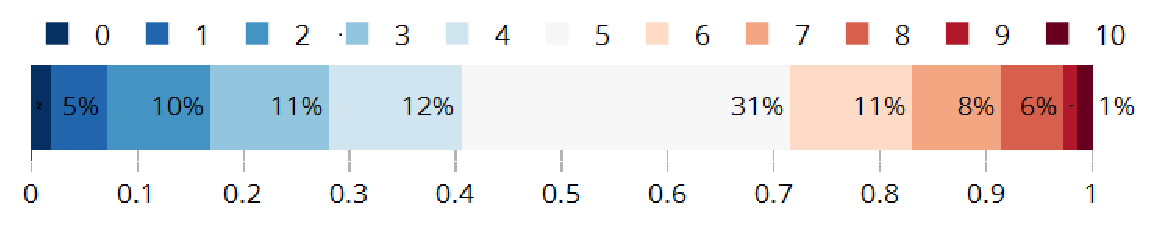
\includegraphics[width=\columnwidth]{Images/CC_target_emission_nolegend.eps}
% \caption{Perceived GhG emission p.c. required in 2050 to limit global warming to +2\textdegree{}C (in tCO$_\textnormal{2}$eq/yr), given that it is now 10.}
% \label{fig:target_emission}
% \end{figure}

%\citet{millner_beliefs_2016} propose several mechanisms to explain people's lack of understanding about climate change: in addition to the difficulty of grasping gradual changes, they emphasize the complexity of drawing a causal link between diffuse causes and distant consequences. Failing to assimilate the underlying channels may blur the link between people's own behavior and consequences for the climate. One related element that may explain why people ignore the basics of climate science is that they do not feel directly affected by CC. 

%In fact, 62\% think that the first generation seriously affected by CC is yet to be born (Figure 5). 

% TODO: Indeed, a delay of one generation as the first affected by CC is significantly associated with a lower knowledge by 0.1 standard deviation, where knowledge is measured by an index formed with the variables presented in this subsection (see Section 6.1) => ça n'apparaît plus ça, c'est où? -> Je ne me rappelle pas non plus...

% email https://cces.gov.harvard.edu/; explore http://closup.umich.edu/national-surveys-on-energy-and-environment/ 
% autre_K:
% ADEME: anthropique/naturel: 71/25 (USA 66/31 Gallup); nucléaire 57% pensent que ça émet assez ou beaucoup de GES, 69% les volcans, 90% (max) activités industrielles
% Leiserowitz 2007: Knowledge around the world, and who should take action. majority in some poor country had never heard about CC in 06, France in average of rich countries https://scholar.google.com/scholar?cluster=7931243904271807197&hl=en&as_sdt=0,5&sciodt=0,5


% \begin{figure}[t]
% \centering
% \includegraphics[width=\columnwidth]{Images/CC_generation_min_nolegend_trim.eps}
% \caption{Perceived date of birth of first generation severely affected by CC.}
% \label{fig:generation}
% \end{figure}

% \begin{figure}[t]
% \centering
% 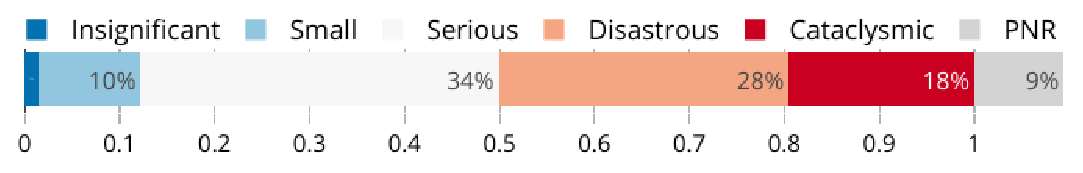
\includegraphics[width=\columnwidth]{Images/CC_effects_nolegend.eps}
% \caption{Perceived gravity of climate change.}
% \label{fig:gravity}
% \end{figure}

% \begin{figure}[b] % !htbp
% \centering
% \includegraphics[width=\columnwidth]{Images/CC_talks_nolegend.eps}
% \caption{Frequency at which respondents talk about climate change.}
% \label{fig:talks}
% \end{figure}


% \begin{figure}[!htbp]
% \centering
% 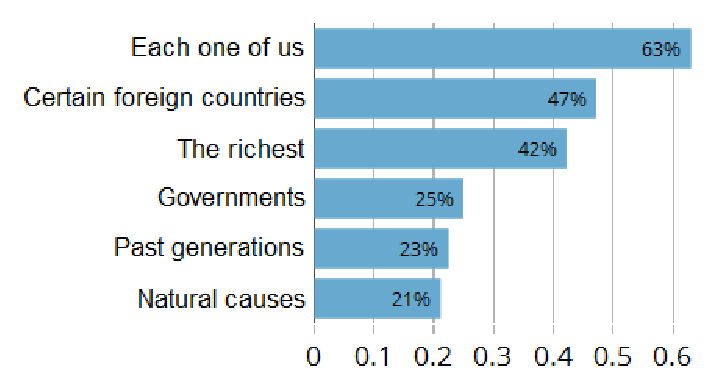
\includegraphics[width=0.75\columnwidth]{Images/CC_responsiblec.eps}
% \caption{Entities perceived responsible for climate change.}
% \label{fig:responsible}
% \end{figure}

% Suggestion!: keep wording after disastrous and grave? 


\
% Note: cite Kahan 2015 for people understands fundamentals

% parle ~ effets
% inquiétude répandue. Qui est tenu responsable.
    
% autre_op: ADEME 63% conditions de vie extrêmement pénibles en France d'ici 50 ans; 57% pensent pas (probablement ou certainement) que le changement climatique sera limité à des niveaux acceptables d’ici à la fin du siècle (similaire à OpinionWay) / A votre avis qui serait le plus efficace pour résoudre le problème du réchauffement climatique ? 35% chacun d'entre nous, 26% états, 14% instances internationales (aux US c'est plus les entreprises, cf Yale)

% Done (footnote ajoutée en section 5): définir "warm glow" -> je ne comprends pas trop pourquoi il nous demande de le définir, mais je suggère de remplacer par : "It may be that people overstate their willingness to do good actions, or lack of knowledge regarding the efforts needed, ..." => je ne trouve pas que "overstate" reflète bien le warm glow car on perd le côté "mauvaise foi" (i.e. mensonge à soi-même), et le "willingness" me semble superflu. Pk pas "overstimate their virtue/goodness"? On utilise aussi "warm glow" ailleurs. On pourrait remplacer par "self-deception", "overconfidence" ou "cheap talk" un des deux mais je crois que préfère rajouter une footnote qui explique ce qu'est le warm glow: \footnote{Here, "warm glow" refers to one's unintentional strategy to overestimate their virtue in order to derive satisfaction.} -> Ok, de toute façon cette section va disparaitre du papier. J'ai inséré la footnote à la deuxième mention du terme.

\section{Test different wording for winners and losers}


\begin{table}[!h] \centering 
  \caption{Effect of defining winners/losers in terms of purchasing power} 
  \label{table:purchasing_power} 
\makebox[\textwidth][c]{ \begin{tabular}{@{\extracolsep{5pt}}lcccc} 
\\[-1.8ex]\hline 
\hline \\[-1.8ex] 
 & \multicolumn{4}{c}{\textit{Dependent variable:}} \\ 
\cline{2-5} 
\\[-1.2ex] & Poors expected & City dwellers expected & Rich expected & Rural expected \\
& to win & to win & to lose & to lose
\\
 & (1) & (2) & (3) & (4) \\ 
\hline \\[-1.8ex] 
 Constant & 0.058$^{***}$ & 0.207$^{***}$ & 0.009$^{***}$ & 0.352$^{***}$ \\ 
  & (0.007) & (0.010) & (0.003) & (0.012) \\ 
  In purchasing power & 0.045$^{***}$ & $-$0.029$^{**}$ & 0.015$^{***}$ & $-$0.014 \\ 
  & (0.010) & (0.014) & (0.005) & (0.017) \\ 
 \hline \\[-1.8ex] 
Observations & 3,002 & 3,002 & 3,002 & 3,002 \\ 
R$^{2}$ & 0.007 & 0.001 & 0.003 & 0.0002 \\ 
\hline 
\hline \\[-1.8ex] 
& \multicolumn{4}{r}{$^{*}$p$<$0.1; $^{**}$p$<$0.05; $^{***}$p$<$0.01} \\ 
\end{tabular} 
} \end{table} 

\clearpage


\section{Additional specifications for determinants of attitudes}

\begin{table*}[!htbp] \centering 
  \caption{Determinants of attitudes towards diesel taxation} 
  \label{tab:determinants_diesel} 
\makebox[\textwidth][c]{ \begin{tabular}{@{\extracolsep{5pt}}lcccc} 
\\[-1.8ex]\hline 
\hline \\[-1.8ex] 
\\[-1.8ex] & \multicolumn{3}{c}{Acceptance increase in diesel taxation} \\ 
\\[-1.8ex] & (1) & (2) & (3) & (4)\\ 
\hline \\[-1.8ex] 
 Knowledge on CC & 0.046$^{***}$ &  &  &  \\ 
  & (0.008) &  &  &  \\ 
  Ecologist & 0.082$^{***}$ &  &  &  \\ 
  & (0.023) &  &  &  \\ 
  Yellow Vests: PNR & $-$0.041 &  & $-$0.068$^{**}$ &  \\ 
  & (0.030) &  & (0.034) &  \\ 
  Yellow Vests: understands & $-$0.099$^{***}$ &  & $-$0.134$^{***}$ &  \\ 
  & (0.021) &  & (0.023) &  \\ 
  Yellow Vests: supports & $-$0.188$^{***}$ &  & $-$0.289$^{***}$ &  \\ 
  & (0.022) &  & (0.024) &  \\ 
  Yellow Vests: is part & $-$0.163$^{***}$ &  & $-$0.300$^{***}$ &  \\ 
  & (0.040) &  & (0.045) &  \\ 
  Left-right: Extreme-left & 0.082 &  &  & 0.076 \\ 
  & (0.052) &  &  & (0.060) \\ 
  Left-right: Left & 0.033 &  &  & 0.025 \\ 
  & (0.025) &  &  & (0.024) \\ 
  Left-right: Center & 0.016 &  &  & 0.081$^{***}$ \\ 
  & (0.028) &  &  & (0.029) \\ 
  Left-right: Right & $-$0.045$^{*}$ &  &  & $-$0.060$^{**}$ \\ 
  & (0.027) &  &  & (0.026) \\ 
  Left-right: Extreme-right & $-$0.030 &  &  & $-$0.180$^{***}$ \\ 
  & (0.031) &  &  & (0.033) \\ 
  Size of town: -20k & $-$0.001 & 0.002 &  &  \\ 
  & (0.025) & (0.025) &  &  \\ 
  Size of town: 20-100k & 0.013 & 0.016 &  &  \\ 
  & (0.027) & (0.027) &  &  \\ 
  Size of town: +100k & 0.068$^{***}$ & 0.106$^{***}$ &  &  \\ 
  & (0.025) & (0.022) &  &  \\ 
  Size of town: Paris & 0.083$^{**}$ & 0.143$^{***}$ &  &  \\ 
  & (0.041) & (0.026) &  &  \\ 
  Diesel & $-$0.371$^{***}$ & $-$0.474$^{***}$ &  &  \\ 
  & (0.023) & (0.016) &  &  \\ 
  Gasoline & 0.153$^{***}$ &  &  &  \\ 
  & (0.022) &  &  &  \\ 
  Number vehicles & $-$0.022 &  &  &  \\ 
  & (0.019) &  &  &  \\ 
  Frequency of public transit & 0.001 &  &  &  \\ 
  & (0.007) &  &  &  \\ 
 \hline \\[-1.8ex] 
Additional covariates & \checkmark &  &  &  \\ 
Observations & 3,002 & 3,002 & 3,002 & 3,002 \\ 
R$^{2}$ & 0.357 & 0.271 & 0.054 & 0.018 \\ 
\hline 
\hline \\[-1.8ex] 
 & \multicolumn{4}{r}{$^{*}$p$<$0.1; $^{**}$p$<$0.05; $^{***}$p$<$0.01} \\ 
\end{tabular} 
} \\ \quad \\ {\footnotesize \textsc{Note:} Standard errors are reported in parentheses. Omitted variables are \textit{Yellow Vests: opposes}, \textit{Age : 18 -- 24} and \textit{Left-right: Indeterminate}. Additional covariates are defined in Appendix C.} \end{table*} 


% Done : shale gas supprimé

% \begin{table}[!h] \centering 
%   \caption{Effect of being treated on acceptance of shale gas exploitation} 
%   \label{table:shale_gas} 
% \makebox[\textwidth][c]{ \begin{tabular}{@{\extracolsep{5pt}}lccc} 
% \\[-1.8ex]\hline 
% \hline \\[.0ex] 
%  & \multicolumn{3}{c}{\textit{Dependent variable: Shale gas exploitation: not ``No''}} \\[.5ex] \cline{2-4} \\[-.5ex]
%  & (1) & (2) & (3) \\
%  \\[-1.8ex] & \textit{OLS} & \textit{OLS} & \textit{logistic} \\ 
% \hline \\[-1.0ex] 
%  District concerned & $-$0.039$^{**}$ & $-$0.054$^{**}$ & $-$0.059$^{**}$ \\ 
%   & (0.019) & (0.024) & (0.024) \\ 
%  \hline \\[-1.0ex] 
% Controls: Socio-demographics, scores &  & \checkmark & \checkmark \\ 
% Observations & 2,847 & 2,847 & 2,847 \\ 
% R$^{2}$ & 0.001 & 0.047 &  \\ 
% \hline 
% \hline \\[-1.8ex] 
% & \multicolumn{3}{r}{$^{*}$p$<$0.1; $^{**}$p$<$0.05; $^{***}$p$<$0.01} \\ 
% \end{tabular} 
% } \end{table} 
% % DONE Treated -> District concerned



\begin{table*}[!htbp] \centering 
  \caption{Determinants of attitudes towards carbon tax revenue recycling} 
  \label{tab:politiques_env} 
\hspace*{-1.3cm} \resizebox{1.15\columnwidth}{!}{ \begin{tabular}{@{\extracolsep{5pt}}lccccccccc} 
\\[-1.8ex]\hline 
\hline \\[-1.8ex] 
\\[-1.8ex] & Non-polluting & VAT & Renewable & Renovation & Transfer & Reduction & Transfer & Reduction & Transfer \\ \\[-1.8ex] & transports & cut & energies & of buildings & constrained hh. & soc. contri. & poor hh. & pub. deficit & all hh. \\ 
\\[-1.8ex] & (1) & (2) & (3) & (4) & (5) & (6) & (7) & (8) & (9)\\ 
\hline \\[-1.8ex] 
 Knowledge on CC & 0.127$^{***}$ & $-$0.050$^{*}$ & 0.132$^{***}$ & 0.099$^{***}$ & 0.051$^{*}$ & $-$0.064$^{**}$ & $-$0.027 & $-$0.009 & $-$0.074$^{**}$ \\ 
  & (0.025) & (0.026) & (0.025) & (0.025) & (0.026) & (0.026) & (0.029) & (0.026) & (0.029) \\ 
  CC is disastrous & 0.298$^{***}$ & 0.085 & 0.275$^{***}$ & 0.247$^{***}$ & 0.151$^{***}$ & 0.109$^{**}$ & 0.102$^{*}$ & 0.105$^{**}$ & 0.078 \\ 
  & (0.049) & (0.052) & (0.050) & (0.049) & (0.052) & (0.053) & (0.057) & (0.052) & (0.057) \\ 
  Interest in politics (0 to 2) & 0.031 & $-$0.115$^{***}$ & $-$0.003 & $-$0.008 & $-$0.006 & $-$0.096$^{**}$ & $-$0.073$^{*}$ & $-$0.079$^{**}$ & $-$0.068$^{*}$ \\ 
  & (0.035) & (0.038) & (0.036) & (0.036) & (0.038) & (0.038) & (0.041) & (0.038) & (0.041) \\ 
  Ecologist & 0.310$^{***}$ & $-$0.036 & 0.436$^{***}$ & 0.262$^{***}$ & 0.055 & $-$0.085 & 0.183$^{**}$ & $-$0.024 & $-$0.012 \\ 
  & (0.068) & (0.073) & (0.069) & (0.068) & (0.072) & (0.073) & (0.078) & (0.072) & (0.079) \\ 
  Yellow Vests: PNR & $-$0.156$^{*}$ & $-$0.041 & $-$0.256$^{***}$ & $-$0.171$^{*}$ & $-$0.140 & $-$0.189$^{**}$ & 0.032 & $-$0.318$^{***}$ & $-$0.129 \\ 
  & (0.089) & (0.096) & (0.091) & (0.090) & (0.095) & (0.096) & (0.104) & (0.095) & (0.104) \\ 
  Yellow Vests: understands & $-$0.039 & 0.262$^{***}$ & $-$0.106$^{*}$ & $-$0.016 & 0.091 & 0.007 & 0.127$^{*}$ & $-$0.096 & $-$0.094 \\ 
  & (0.061) & (0.066) & (0.062) & (0.061) & (0.065) & (0.066) & (0.071) & (0.065) & (0.071) \\ 
  Yellow Vests: supports & $-$0.271$^{***}$ & 0.141$^{**}$ & $-$0.346$^{***}$ & $-$0.243$^{***}$ & $-$0.098 & $-$0.166$^{**}$ & $-$0.043 & $-$0.321$^{***}$ & $-$0.277$^{***}$ \\ 
  & (0.065) & (0.070) & (0.066) & (0.065) & (0.069) & (0.070) & (0.076) & (0.069) & (0.076) \\ 
  Yellow Vests: is part & $-$0.306$^{***}$ & 0.272$^{**}$ & $-$0.370$^{***}$ & $-$0.211$^{*}$ & 0.022 & $-$0.112 & $-$0.023 & $-$0.297$^{**}$ & $-$0.345$^{**}$ \\ 
  & (0.118) & (0.127) & (0.120) & (0.119) & (0.126) & (0.127) & (0.137) & (0.125) & (0.137) \\ 
  Left-right: Extreme-left & 0.066 & 0.162 & 0.066 & 0.223 & 0.043 & $-$0.195 & 0.180 & $-$0.216 & $-$0.399$^{**}$ \\ 
  & (0.154) & (0.166) & (0.157) & (0.155) & (0.164) & (0.166) & (0.179) & (0.164) & (0.179) \\ 
  Left-right: Left & 0.085 & $-$0.079 & 0.145$^{*}$ & 0.089 & 0.074 & $-$0.097 & 0.301$^{***}$ & $-$0.099 & $-$0.065 \\ 
  & (0.074) & (0.080) & (0.076) & (0.075) & (0.079) & (0.080) & (0.086) & (0.079) & (0.087) \\ 
  Left-right: Center & 0.038 & $-$0.162$^{*}$ & 0.021 & 0.137$^{*}$ & 0.083 & $-$0.093 & 0.054 & 0.105 & $-$0.100 \\ 
  & (0.082) & (0.088) & (0.084) & (0.083) & (0.087) & (0.089) & (0.095) & (0.087) & (0.096) \\ 
  Left-right: Right & 0.048 & $-$0.013 & 0.058 & 0.084 & 0.072 & 0.090 & $-$0.134 & 0.160$^{*}$ & 0.051 \\ 
  & (0.079) & (0.085) & (0.080) & (0.079) & (0.084) & (0.085) & (0.092) & (0.084) & (0.092) \\ 
  Left-right: Extreme-right & $-$0.212$^{**}$ & $-$0.041 & $-$0.106 & $-$0.147 & $-$0.186$^{*}$ & $-$0.013 & $-$0.209$^{*}$ & $-$0.172$^{*}$ & $-$0.095 \\ 
  & (0.093) & (0.100) & (0.095) & (0.094) & (0.099) & (0.100) & (0.108) & (0.099) & (0.108) \\ 
  Diploma (1 to 4) & $-$0.014 & $-$0.027 & 0.016 & 0.002 & $-$0.014 & $-$0.047$^{*}$ & $-$0.046 & $-$0.021 & 0.011 \\ 
  & (0.025) & (0.026) & (0.025) & (0.025) & (0.026) & (0.027) & (0.029) & (0.026) & (0.029) \\ 
  Age: 25 -- 34 & $-$0.285$^{**}$ & $-$0.105 & $-$0.270$^{**}$ & $-$0.101 & $-$0.096 & $-$0.120 & $-$0.308$^{**}$ & $-$0.261$^{**}$ & 0.244$^{*}$ \\ 
  & (0.113) & (0.121) & (0.115) & (0.113) & (0.120) & (0.121) & (0.131) & (0.120) & (0.131) \\ 
  Age: 35 -- 49 & $-$0.167 & $-$0.083 & $-$0.109 & 0.057 & $-$0.023 & 0.014 & $-$0.283$^{**}$ & $-$0.202$^{*}$ & 0.096 \\ 
  & (0.112) & (0.120) & (0.114) & (0.112) & (0.119) & (0.120) & (0.130) & (0.119) & (0.130) \\ 
  Age: 50 -- 64 & $-$0.015 & 0.032 & $-$0.038 & 0.122 & 0.178 & 0.166 & $-$0.053 & $-$0.176 & 0.129 \\ 
  & (0.121) & (0.130) & (0.124) & (0.122) & (0.129) & (0.131) & (0.141) & (0.129) & (0.141) \\ 
  Age: $\geq$ 65 & $-$0.010 & $-$0.034 & $-$0.034 & 0.217 & 0.215 & 0.130 & 0.028 & $-$0.140 & 0.111 \\ 
  & (0.143) & (0.154) & (0.146) & (0.144) & (0.152) & (0.154) & (0.166) & (0.152) & (0.166) \\ 
  Income (k\euro{}/month) & 0.025 & $-$0.016 & 0.014 & 0.013 & $-$0.014 & $-$0.002 & $-$0.084$^{***}$ & 0.008 & 0.054$^{**}$ \\ 
  & (0.022) & (0.023) & (0.022) & (0.022) & (0.023) & (0.023) & (0.025) & (0.023) & (0.025) \\ 
  Sex: Male & $-$0.151$^{***}$ & $-$0.183$^{***}$ & $-$0.183$^{***}$ & $-$0.132$^{***}$ & $-$0.190$^{***}$ & $-$0.221$^{***}$ & $-$0.161$^{***}$ & $-$0.132$^{**}$ & $-$0.108$^{*}$ \\ 
  & (0.049) & (0.053) & (0.050) & (0.049) & (0.052) & (0.053) & (0.057) & (0.052) & (0.057) \\ 
  Size of town (1 to 5) & $-$0.007 & 0.005 & 0.004 & 0.003 & $-$0.012 & 0.019 & 0.029 & 0.016 & $-$0.007 \\ 
  & (0.021) & (0.023) & (0.022) & (0.021) & (0.023) & (0.023) & (0.025) & (0.023) & (0.025) \\ 
  Frequency of public transit & 0.025 & $-$0.026 & $-$0.006 & 0.0001 & $-$0.012 & $-$0.015 & $-$0.019 & $-$0.029 & $-$0.014 \\ 
  & (0.020) & (0.022) & (0.021) & (0.021) & (0.022) & (0.022) & (0.024) & (0.022) & (0.024) \\ 
 \hline \\[-1.8ex] 
Additional covariates & \checkmark & \checkmark & \checkmark  & \checkmark & \checkmark & \checkmark & \checkmark & \checkmark & \checkmark \\ 
Observations & 3,002 & 3,002 & 3,002 & 3,002 & 3,002 & 3,002 & 3,002 & 3,002 & 3,002 \\ 
R$^{2}$ & 0.125 & 0.066 & 0.129 & 0.095 & 0.060 & 0.058 & 0.120 & 0.053 & 0.064 \\ 
\hline 
\hline \\[-1.8ex] 
& \multicolumn{9}{r}{$^{*}$p$<$0.1; $^{**}$p$<$0.05; $^{***}$p$<$0.01} \\ 
\end{tabular} 
} \\ \quad \\ {\footnotesize \textsc{Note:} Standard errors are reported in parentheses. Omitted variables are \textit{Yellow Vests: opposes}, \textit{Age : 18 -- 24} and \textit{Left-right: Indeterminate}. Additional covariates are defined in Appendix C.} \end{table*} 


\clearpage


\begin{table*}[!htbp] \centering 
  \caption{Determinants of attitudes towards specific climate policies} 
  \label{tab:politiques_env} 
\hspace*{-1.3cm} \resizebox{1.15\columnwidth}{!}{ \begin{tabular}{@{\extracolsep{5pt}}lcccccccc} 
\\[-1.8ex]\hline 
\hline \\[-1.8ex] 
\\[-1.8ex] & Norms for & Norms for & Tax on & Prohibition & Norms for & Contribution & Tax on & Urban \\ \\[-1.8ex] & buildings & new vehicles & kerosene & pol. vehicles & old vehicles & climate fund & red meat & tolls \\ 
\\[-1.8ex] & (1) & (2) & (3) & (4) & (5) & (6) & (7) & (8)\\ 
\hline \\[-1.8ex] 
 Knowledge on CC & 0.155$^{***}$ & 0.186$^{***}$ & 0.130$^{***}$ & 0.118$^{***}$ & 0.100$^{***}$ & 0.187$^{***}$ & 0.118$^{***}$ & 0.027 \\ 
  & (0.022) & (0.022) & (0.024) & (0.025) & (0.024) & (0.025) & (0.023) & (0.023) \\ 
  CC is disastrous & 0.175$^{***}$ & 0.360$^{***}$ & 0.105$^{**}$ & 0.246$^{***}$ & 0.252$^{***}$ & 0.271$^{***}$ & 0.160$^{***}$ & 0.092$^{**}$ \\ 
  & (0.043) & (0.043) & (0.047) & (0.050) & (0.047) & (0.050) & (0.046) & (0.046) \\ 
  Interest in politics (0 to 2) & 0.117$^{***}$ & 0.115$^{***}$ & 0.245$^{***}$ & 0.022 & 0.003 & 0.041 & $-$0.022 & 0.027 \\ 
  & (0.031) & (0.031) & (0.034) & (0.036) & (0.034) & (0.036) & (0.033) & (0.033) \\ 
  Ecologist & 0.141$^{**}$ & 0.160$^{***}$ & 0.263$^{***}$ & 0.317$^{***}$ & 0.233$^{***}$ & 0.288$^{***}$ & 0.480$^{***}$ & 0.267$^{***}$ \\ 
  & (0.059) & (0.059) & (0.065) & (0.069) & (0.066) & (0.069) & (0.063) & (0.064) \\ 
  Yellow Vests: PNR & $-$0.151$^{*}$ & $-$0.084 & $-$0.203$^{**}$ & $-$0.104 & $-$0.127 & $-$0.086 & 0.012 & $-$0.213$^{**}$ \\ 
  & (0.078) & (0.078) & (0.086) & (0.091) & (0.087) & (0.091) & (0.083) & (0.084) \\ 
  Yellow Vests: understands & $-$0.005 & $-$0.103$^{*}$ & 0.041 & $-$0.162$^{***}$ & $-$0.139$^{**}$ & $-$0.113$^{*}$ & 0.069 & $-$0.224$^{***}$ \\ 
  & (0.053) & (0.053) & (0.059) & (0.062) & (0.059) & (0.062) & (0.057) & (0.058) \\ 
  Yellow Vests: supports & $-$0.071 & $-$0.178$^{***}$ & 0.201$^{***}$ & $-$0.285$^{***}$ & $-$0.294$^{***}$ & $-$0.291$^{***}$ & 0.059 & $-$0.365$^{***}$ \\ 
  & (0.057) & (0.057) & (0.062) & (0.066) & (0.063) & (0.066) & (0.061) & (0.061) \\ 
  Yellow Vests: is part & $-$0.147 & $-$0.447$^{***}$ & 0.171 & $-$0.573$^{***}$ & $-$0.456$^{***}$ & $-$0.536$^{***}$ & $-$0.107 & $-$0.324$^{***}$ \\ 
  & (0.104) & (0.103) & (0.113) & (0.121) & (0.115) & (0.120) & (0.111) & (0.112) \\ 
  Left-right: Extreme-left & $-$0.076 & $-$0.174 & 0.007 & $-$0.191 & $-$0.051 & 0.267$^{*}$ & 0.199 & $-$0.017 \\ 
  & (0.135) & (0.135) & (0.148) & (0.157) & (0.150) & (0.157) & (0.144) & (0.146) \\ 
  Left-right: Left & 0.009 & $-$0.067 & $-$0.070 & $-$0.084 & $-$0.110 & 0.226$^{***}$ & $-$0.007 & 0.056 \\ 
  & (0.065) & (0.065) & (0.071) & (0.076) & (0.072) & (0.076) & (0.070) & (0.070) \\ 
  Left-right: Center & 0.062 & $-$0.017 & 0.111 & $-$0.043 & 0.029 & $-$0.047 & 0.028 & 0.110 \\ 
  & (0.072) & (0.072) & (0.079) & (0.084) & (0.080) & (0.084) & (0.077) & (0.078) \\ 
  Left-right: Right & $-$0.046 & $-$0.036 & $-$0.048 & $-$0.021 & 0.003 & $-$0.047 & $-$0.114 & 0.009 \\ 
  & (0.069) & (0.069) & (0.076) & (0.080) & (0.077) & (0.080) & (0.074) & (0.074) \\ 
  Left-right: Extreme-right & $-$0.013 & $-$0.064 & 0.007 & $-$0.215$^{**}$ & $-$0.262$^{***}$ & $-$0.329$^{***}$ & $-$0.236$^{***}$ & $-$0.180$^{**}$ \\ 
  & (0.082) & (0.082) & (0.089) & (0.095) & (0.090) & (0.095) & (0.087) & (0.088) \\ 
  Diploma (1 to 4) & $-$0.030 & $-$0.003 & 0.017 & 0.044$^{*}$ & 0.015 & $-$0.037 & 0.011 & 0.016 \\ 
  & (0.022) & (0.022) & (0.024) & (0.025) & (0.024) & (0.025) & (0.023) & (0.023) \\ 
  Age: 25 -- 34 & $-$0.012 & $-$0.066 & 0.223$^{**}$ & 0.051 & $-$0.015 & $-$0.174 & $-$0.199$^{*}$ & $-$0.016 \\ 
  & (0.099) & (0.099) & (0.108) & (0.115) & (0.109) & (0.115) & (0.105) & (0.106) \\ 
  Age: 35 -- 49 & $-$0.014 & 0.087 & 0.319$^{***}$ & 0.130 & $-$0.060 & $-$0.227$^{**}$ & $-$0.419$^{***}$ & $-$0.155 \\ 
  & (0.098) & (0.098) & (0.107) & (0.114) & (0.109) & (0.114) & (0.105) & (0.106) \\ 
  Age: 50 -- 64 & 0.096 & 0.145 & 0.427$^{***}$ & 0.173 & 0.090 & $-$0.368$^{***}$ & $-$0.423$^{***}$ & $-$0.199$^{*}$ \\ 
  & (0.106) & (0.106) & (0.116) & (0.124) & (0.118) & (0.123) & (0.113) & (0.114) \\ 
  Age: $\geq$ 65 & 0.080 & 0.123 & 0.447$^{***}$ & 0.275$^{*}$ & 0.210 & $-$0.483$^{***}$ & $-$0.394$^{***}$ & $-$0.109 \\ 
  & (0.125) & (0.125) & (0.137) & (0.146) & (0.139) & (0.145) & (0.134) & (0.135) \\ 
  Income (k\euro{}/month) & 0.029 & 0.004 & $-$0.025 & 0.040$^{*}$ & 0.038$^{*}$ & 0.039$^{*}$ & 0.004 & 0.046$^{**}$ \\ 
  & (0.019) & (0.019) & (0.021) & (0.022) & (0.021) & (0.022) & (0.020) & (0.020) \\ 
  Sex: Male & $-$0.120$^{***}$ & $-$0.114$^{***}$ & 0.057 & $-$0.026 & $-$0.132$^{***}$ & $-$0.216$^{***}$ & $-$0.136$^{***}$ & $-$0.002 \\ 
  & (0.043) & (0.043) & (0.047) & (0.050) & (0.047) & (0.050) & (0.046) & (0.046) \\ 
  Size of town (1 to 5) & 0.003 & 0.004 & $-$0.041$^{**}$ & 0.020 & 0.018 & 0.038$^{*}$ & 0.049$^{**}$ & $-$0.029 \\ 
  & (0.019) & (0.019) & (0.020) & (0.022) & (0.021) & (0.022) & (0.020) & (0.020) \\ 
  Frequency of public transit & 0.013 & 0.002 & $-$0.040$^{**}$ & $-$0.028 & $-$0.002 & $-$0.040$^{*}$ & $-$0.052$^{***}$ & $-$0.036$^{*}$ \\ 
  & (0.018) & (0.018) & (0.020) & (0.021) & (0.020) & (0.021) & (0.019) & (0.019) \\ 

 \hline \\[-1.8ex] 
Additional covariates & \checkmark & \checkmark & \checkmark & \checkmark & \checkmark & \checkmark & \checkmark & \checkmark \\ 
Observations & 3,002 & 3,002 & 3,002 & 3,002 & 3,002 & 3,002 & 3,002 & 3,002 \\ 
R$^{2}$ & 0.086 & 0.165 & 0.117 & 0.164 & 0.176 & 0.173 & 0.147 & 0.118 \\ 
\hline 
\hline \\[-1.8ex] 
& \multicolumn{8}{r}{$^{*}$p$<$0.1; $^{**}$p$<$0.05; $^{***}$p$<$0.01} \\ 
\end{tabular} 
} \\ \quad \\ {\footnotesize \textsc{Note:} Standard errors are reported in parentheses. Omitted variables are \textit{Yellow Vests: opposes}, \textit{Age : 18 -- 24} and \textit{Left-right: Indeterminate}. Additional covariates are defined in Appendix C.} \end{table*} 


 \clearpage

\begin{table*}[!htbp] \centering 
  \caption{Determinants of attitudes towards climate policies, additional specifications} 
  \label{tab:politiques_env} 
\makebox[\textwidth][c]{ \begin{tabular}{@{\extracolsep{5pt}}lccc} 
\\[-1.8ex]\hline 
\hline \\[-1.8ex] 
\\[-1.8ex] & Share of policies & \multicolumn{2}{c}{Tax \& dividend} \\ 
\\[-1.8ex] & (1) & (2) & (3)\\ 
\hline \\[-1.8ex] 
 Knowledge on CC & 0.057$^{***}$ &  &  \\ 
  & (0.005) &  &  \\ 
  CC is disastrous & 0.090$^{***}$ &  &  \\ 
  & (0.010) &  &  \\ 
  Diploma (1 to 4) & 0.006 &  &  \\ 
  & (0.004) &  &  \\ 
  Age: 25 -- 34 & $-$0.039$^{**}$ &  &  \\ 
  & (0.018) &  &  \\ 
  Age: 35 -- 49 & $-$0.019 &  &  \\ 
  & (0.017) &  &  \\ 
  Age: 50 -- 64 & 0.005 &  &  \\ 
  & (0.017) &  &  \\ 
  Age: $\geq$ 65 & 0.045$^{**}$ &  &  \\ 
  & (0.018) &  &  \\ 
  Income (k\euro{}/month) & 0.003 &  &  \\ 
  & (0.002) &  &  \\ 
  Sex: Male & $-$0.008 &  &  \\ 
  & (0.009) &  &  \\ 
  Size of town (1 to 5) & 0.008$^{**}$ &  &  \\ 
  & (0.004) &  &  \\ 
  Frequency of public transit & 0.017$^{***}$ &  &  \\ 
  & (0.004) &  &  \\ 
  Left-right: Extreme-left &  & 0.072$^{**}$ & $-$0.065 \\ 
  &  & (0.033) & (0.057) \\ 
  Left-right: Left &  & 0.040$^{***}$ & 0.031 \\ 
  &  & (0.013) & (0.022) \\ 
  Left-right: Center &  & 0.071$^{***}$ & 0.090$^{***}$ \\ 
  &  & (0.015) & (0.026) \\ 
  Left-right: Right &  & 0.029$^{**}$ & $-$0.037 \\ 
  &  & (0.014) & (0.024) \\ 
  Left-right: Extreme-right &  & $-$0.061$^{***}$ & $-$0.155$^{***}$ \\ 
  &  & (0.018) & (0.031) \\ 
 \hline \\[-1.8ex] 
Observations & 3,002 & 3,002 & 3,002 \\ 
R$^{2}$ & 0.143 & 0.018 & 0.017 \\ 
\hline 
\hline \\[-1.8ex] 
& \multicolumn{3}{r}{$^{*}$p$<$0.1; $^{**}$p$<$0.05; $^{***}$p$<$0.01} \\ 
\end{tabular} 
} \\ \quad \\ {\footnotesize \textsc{Note:} Standard errors are reported in parentheses. Omitted variables are \textit{Yellow Vests: opposes}, \textit{Age : 18 -- 24} and \textit{Left-right: Indeterminate}. Additional covariates are defined in Appendix C.} \end{table*} 


\clearpage



\section{Construction of the knowledge index}

% newdone : j'ai coupé ici et déplacé dans le texte principal. La seule chose qui a complètement disparu c'est la référence à Tobler (on en parle simplement au relecteur dans la lettre). Je pense que ce n'est pas utile de préciser la valeur du Cronbach puisque cette mesure n'est pas pertinente ici.

%As shown by \citet{kiel_einfuhrung_2002} and summarized by \citet{hoppe_what_2018}, one can distinguish different kinds of knowledge relative to climate change, including causal knowledge (notably about the anthropogenic origin), basic knowledge (about climate science), effects knowledge (about the impacts) and action-related knowledge (about the factors of CC). \footnote{\citet{tobler_et_al_2012} propose different scales to test different aspects of knowledge or perceptions of CC. If each of their scale is reliable (with a relatively high Cronbach's $\alpha$), their scales are not meant to be aggregated. On the contrary, we aim at synthesizing the different aspects of knowledge about CC in one index. Thus, it is no surprise if our index is not highly reliable, as it adds up questions that measures these different aspects. For that matter, we find a Cronbach's $\alpha$ of 0.25).} We synthesize these different dimensions of knowledge using our questions on the existence and anthropogenic origin of CC (corresponding to the causal knowledge), on the region most affected (effects), as well as our scores on the emission target (basic), greenhouse gases (basic) and on activities responsible for CC (action-related). 

We synthesize the different dimensions of knowledge proposed by \citet{kiel_einfuhrung_2002} and summarized by \citet{hoppe_what_2018} using our questions on the existence and anthropogenic origin of CC (corresponding to the causal knowledge), on the region most affected (effects), as well as our scores on the emission target (basic), greenhouse gases (basic) and on activities responsible for CC (action-related).


From an exploratory factor analysis (fitted using the maximum likelihood method), we find the factor which explains the highest share of common variance, and report it in Table \ref{table:loadings}. We use the factor loadings hereby obtained to define the relative weights of the components of our index of knowledge, and we round them for readability purpose. The rounding has virtually no effect on the result, as the correlation between our index and the factor obtained is 0.999. For information, the correlations between the different components of our index, including our index itself, are reported on Figure \ref{fig:correlations_K}.

Moreover, Table \ref{tab:robust_K} shows that the determinants of Tax \& Dividend are robust to the choice of the \textit{knowledge} variable: if we replace our index by any of its component, the coefficients of the other determinants are virtually unchanged. Interestingly, this analysis indicates that it is the knowledge on the existence and the anthropogenic nature of CC that drives the effect of overall knowledge, justifying a higher weight for these two components. Finally, we could reproduce this robustness check for the other dependent variable of Table II, and also by replacing the independent variable \textit{knowledge} in Table I, and we would again see that the other coefficients are essentially unaffected.

\begin{table}[!h] \centering 
  \caption{Factor loadings and weights chosen for different dimensions of knowledge on CC} 
  \label{table:loadings} 
\makebox[\textwidth][c]{ \begin{tabular}{@{\extracolsep{5pt}}lcccccc} 

\textbf{Variable} & GhG & Activities & Exists & Anthropogenic & Target & Region \\  
\hline \\[-1.8ex] 
\textbf{Loading} & .212 & .182 & .398 & .601 & .200 & .000 \\
\textbf{Weight} & 1 & 1 & 2 & 3 & 1 & 0 \\
\end{tabular} 
} \end{table} 

\begin{figure}[!htbp]
\centering
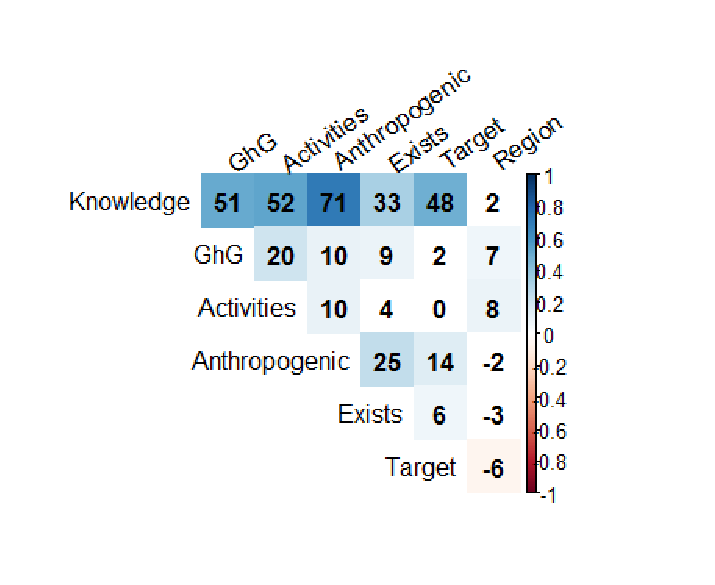
\includegraphics[width=0.51\columnwidth]{correlations_knowledge.eps}
\caption{Correlations between different variables of knowledge on CC.}
\label{fig:correlations_K}
\end{figure}

\begin{table*}[!htbp] \centering 
  \caption{Robustness of the determinants of Tax \& Dividend Acceptance To Knowledge Variables} 
  \label{tab:robust_K} 
\makebox[\textwidth][c]{ \begin{tabular}{@{\extracolsep{5pt}}lcccccc} 
\\[-1.8ex]\hline 
\hline \\[-1.8ex] 
\\[-1.8ex] & \multicolumn{6}{c}{Tax \& dividend} \\ 
\\[-1.8ex] & (1) & (2) & (3) & (4) & (5) & (6)\\ 
\hline \\[-1.8ex] 
 Knowledge on CC & 0.029$^{***}$ &  &  &  &  &  \\ 
  & (0.009) &  &  &  &  &  \\ 
  CC is Anthropogenic &  & 0.068$^{***}$ &  &  &  &  \\ 
  &  & (0.019) &  &  &  &  \\ 
  CC Exists &  &  & 0.115$^{**}$ &  &  &  \\ 
  &  &  & (0.051) &  &  &  \\ 
  Score GhG &  &  &  & 0.002 &  &  \\ 
  &  &  &  & (0.009) &  &  \\ 
  Score Activities &  &  &  &  & 0.005 &  \\ 
  &  &  &  &  & (0.009) &  \\ 
  Score Target proximity &  &  &  &  &  & 0.015$^{*}$ \\ 
  &  &  &  &  &  & (0.008) \\ 
  Ecologist & 0.126$^{***}$ & 0.130$^{***}$ & 0.135$^{***}$ & 0.135$^{***}$ & 0.134$^{***}$ & 0.132$^{***}$ \\ 
  & (0.024) & (0.024) & (0.024) & (0.024) & (0.024) & (0.024) \\ 
  Yellow Vests: PNR & $-$0.021 & $-$0.019 & $-$0.023 & $-$0.023 & $-$0.023 & $-$0.024 \\ 
  & (0.032) & (0.032) & (0.032) & (0.032) & (0.032) & (0.032) \\ 
  Yellow Vests: understands & $-$0.144$^{***}$ & $-$0.144$^{***}$ & $-$0.146$^{***}$ & $-$0.146$^{***}$ & $-$0.145$^{***}$ & $-$0.146$^{***}$ \\ 
  & (0.022) & (0.022) & (0.022) & (0.022) & (0.022) & (0.022) \\ 
  Yellow Vests: supports & $-$0.222$^{***}$ & $-$0.222$^{***}$ & $-$0.226$^{***}$ & $-$0.228$^{***}$ & $-$0.227$^{***}$ & $-$0.227$^{***}$ \\ 
  & (0.023) & (0.023) & (0.023) & (0.023) & (0.023) & (0.023) \\ 
  Yellow Vests: is part & $-$0.214$^{***}$ & $-$0.215$^{***}$ & $-$0.218$^{***}$ & $-$0.226$^{***}$ & $-$0.225$^{***}$ & $-$0.225$^{***}$ \\ 
  & (0.043) & (0.043) & (0.043) & (0.042) & (0.043) & (0.042) \\ 
  Left-right: Extreme-left & $-$0.040 & $-$0.038 & $-$0.028 & $-$0.033 & $-$0.033 & $-$0.037 \\ 
  & (0.056) & (0.056) & (0.056) & (0.056) & (0.056) & (0.056) \\ 
  Left-right: Left & 0.072$^{***}$ & 0.072$^{***}$ & 0.075$^{***}$ & 0.075$^{***}$ & 0.074$^{***}$ & 0.075$^{***}$ \\ 
  & (0.027) & (0.027) & (0.027) & (0.027) & (0.027) & (0.027) \\ 
  Left-right: Center & 0.051$^{*}$ & 0.053$^{*}$ & 0.052$^{*}$ & 0.053$^{*}$ & 0.053$^{*}$ & 0.054$^{*}$ \\ 
  & (0.030) & (0.030) & (0.030) & (0.030) & (0.030) & (0.030) \\ 
  Left-right: Right & $-$0.022 & $-$0.022 & $-$0.023 & $-$0.023 & $-$0.023 & $-$0.022 \\ 
  & (0.028) & (0.028) & (0.028) & (0.028) & (0.028) & (0.028) \\ 
  Left-right: Extreme-right & $-$0.041 & $-$0.044 & $-$0.046 & $-$0.045 & $-$0.044 & $-$0.045 \\ 
  & (0.034) & (0.034) & (0.034) & (0.034) & (0.034) & (0.034) \\ 
  Sex: Male & $-$0.053$^{***}$ & $-$0.047$^{***}$ & $-$0.046$^{***}$ & $-$0.048$^{***}$ & $-$0.049$^{***}$ & $-$0.048$^{***}$ \\ 
  & (0.018) & (0.018) & (0.018) & (0.018) & (0.018) & (0.018) \\ 
 \hline \\[-1.8ex] 
Additional covariates & \checkmark & & \checkmark  & \checkmark & \checkmark & \checkmark  \\ 
Observations & 3,002 & 3,002 & 3,002 & 3,002 & 3,002 & 3,002 \\ 
R$^{2}$ & 0.150 & 0.151 & 0.149 & 0.147 & 0.147 & 0.148 \\ 
\hline 
\hline \\[-1.8ex] 
& \multicolumn{6}{r}{$^{*}$p$<$0.1; $^{**}$p$<$0.05; $^{***}$p$<$0.01} \\ 
\end{tabular} 
} \\ \quad \\ {\footnotesize \textsc{Note:} Standard errors are reported in parentheses. Omitted variables are \textit{Yellow Vests: opposes}, \textit{Age : 18 -- 24} and \textit{Left-right: Indeterminate}. Additional covariates are the same as in Table II.} \end{table*} 

\clearpage


\section{Logit regressions for determinants}


\vspace{-0.5cm}

\begin{table*}[!htbp] \centering 
  \caption{Determinants of attitudes towards climate change (CC) with logit regressions.} 
  \label{tab:determinants_attitudes_CC} 
\makebox[\textwidth][c]{ \resizebox{.86\columnwidth}{!}{ \begin{tabular}{@{\extracolsep{5pt}}lccccc} 
\\[-1.8ex]\hline 
\hline \\[-1.8ex] 
\\[-1.8ex] & \multicolumn{3}{c}{CC is anthropogenic} & \multicolumn{2}{c}{CC is disastrous} \\ 
\\[-1.8ex] & (1) & (2) & (3) & (4) & (5)\\ 
\hline \\[-1.8ex] 
 Interest in politics (0 to 2) & 0.034$^{***}$ &  &  & 0.045$^{***}$ &  \\ 
  & (0.013) &  &  & (0.014) &  \\ 
  Ecologist & 0.144$^{***}$ &  &  & 0.186$^{***}$ &  \\ 
  & (0.021) &  &  & (0.027) &  \\ 
  Yellow Vests: PNR & $-$0.097$^{***}$ &  &  & $-$0.069$^{**}$ &  \\ 
  & (0.036) &  &  & (0.034) &  \\ 
  Yellow Vests: understands & $-$0.034 &  &  & $-$0.040$^{*}$ &  \\ 
  & (0.023) &  &  & (0.024) &  \\ 
  Yellow Vests: supports & $-$0.101$^{***}$ &  &  & $-$0.052$^{**}$ &  \\ 
  & (0.025) &  &  & (0.025) &  \\ 
  Yellow Vests: is part & $-$0.196$^{***}$ &  &  & $-$0.079$^{*}$ &  \\ 
  & (0.047) &  &  & (0.044) &  \\ 
  Left-right: Extreme-left & 0.121$^{**}$ &  & 0.079 & 0.070 & 0.006 \\ 
  & (0.047) &  & (0.071) & (0.064) & (0.088) \\ 
  Left-right: Left & 0.088$^{***}$ &  & 0.050 & 0.104$^{***}$ & $-$0.006 \\ 
  & (0.025) &  & (0.045) & (0.030) & (0.053) \\ 
  Left-right: Center & 0.011 &  & 0.009 & 0.030 & $-$0.072 \\ 
  & (0.030) &  & (0.044) & (0.032) & (0.048) \\ 
  Left-right: Right & $-$0.031 &  & $-$0.032 & $-$0.029 & $-$0.138$^{***}$ \\ 
  & (0.029) &  & (0.046) & (0.031) & (0.048) \\ 
  Left-right: Extreme-right & $-$0.012 &  & $-$0.025 & 0.023 & $-$0.081 \\ 
  & (0.034) &  & (0.056) & (0.038) & (0.062) \\ 
  Diploma: \textit{CAP} or \textit{BEP} & 0.042$^{**}$ &  & 0.039$^{*}$ & $-$0.022 & $-$0.015 \\ 
  & (0.020) &  & (0.021) & (0.025) & (0.026) \\ 
  Diploma: \textit{Baccalauréat} & 0.063$^{***}$ &  & 0.111$^{***}$ & 0.025 & 0.121$^{***}$ \\ 
  & (0.024) &  & (0.024) & (0.029) & (0.030) \\ 
  Diploma: Higher & 0.093$^{***}$ &  & 0.165$^{***}$ & 0.095$^{***}$ & 0.234$^{***}$ \\ 
  & (0.025) &  & (0.024) & (0.031) & (0.030) \\ 
  Diploma $\times$ Left-right &  &  & $-$0.010 &  & $-$0.004 \\ 
  &  &  & (0.008) &  & (0.009) \\ 
  Diploma $\times$ Left-right: Indeterminate &  &  & 0.005 &  & $-$0.024 \\ 
  &  &  & (0.015) &  & (0.016) \\   
  Age: 25 -- 34 & 0.048 & $-$0.040 &  & 0.018 &  \\ 
  & (0.042) & (0.041) &  & (0.047) &  \\ 
  Age: 35 -- 49 & $-$0.008 & $-$0.113$^{***}$ &  & 0.026 &  \\ 
  & (0.043) & (0.035) &  & (0.045) &  \\ 
  Age: 50 -- 64 & 0.005 & $-$0.116$^{***}$ &  & $-$0.036 &  \\ 
  & (0.045) & (0.034) &  & (0.047) &  \\ 
  Age: $\geq$ 65 & $-$0.095$^{*}$ & $-$0.228$^{***}$ &  & $-$0.087 &  \\ 
  & (0.057) & (0.035) &  & (0.056) &  \\ 
  Income (k\euro{}/month) & $-$0.011 &  &  & $-$0.010 &  \\ 
  & (0.008) &  &  & (0.009) &  \\ 
  Sex: Male & $-$0.024 &  &  & 0.003 &  \\ 
  & (0.018) &  &  & (0.019) &  \\ 
  Size of town (1 to 5) & 0.006 &  &  & 0.007 &  \\ 
  & (0.008) &  &  & (0.008) &  \\ 
  Frequency of public transit & 0.012 &  &  & 0.007 &  \\ 
  & (0.007) &  &  & (0.008) &  \\ 
 \hline \\[-1.8ex] 
Additional covariates & \checkmark &  &  & \checkmark &  \\  &  &  &  &  &  \\ 
Observations & 3,002 & 3,002 & 3,002 & 3,002 & 3,002 \\ 
\hline 
\hline \\[-1.8ex] 
\textit{Note:}  & \multicolumn{5}{r}{$^{*}$p$<$0.1; $^{**}$p$<$0.05; $^{***}$p$<$0.01} \\ 
\end{tabular} }
}{\\ $\quad$ \\                \footnotesize \textsc{Note:} Standard errors are reported in parentheses. Interaction term is computed using numeric variables. Omitted modalities are: \textit{Yellow Vests: opposes}, \textit{Left-right: Indeterminate}, \textit{Diploma: Brevet or no diploma}, \textit{Age: 18 -- 24}. Additional covariates are defined in Appendix C. }                \end{table*}  
% Note: Table 5.1 de l'OA, on a toujours 1813 obs, les "Indeterminate" sont exclus.. Même chose à la table 6.1



\begin{table*}[!htbp] \centering 
  \caption{Determinants of attitudes towards climate policies with logit regressions.} 
  \label{tab:politiques_env_logit} 
\makebox[\textwidth][c]{ \begin{tabular}{@{\extracolsep{5pt}}lcccc} 
\\[-1.8ex]\hline 
\hline \\[-1.8ex] 
\\[-1.8ex] & \multicolumn{2}{c}{Tax \& dividend} & Share of policies & Ecological lifestyle \\ 
\\[-1.8ex] & (1) & (2) & (3) & (4)\\ 
\hline \\[-1.8ex] 
 Knowledge on CC & 0.029$^{***}$ & 0.049$^{***}$ & 0.046$^{***}$ & 0.092$^{***}$ \\ 
  & (0.009) & (0.009) & (0.010) & (0.010) \\ 
  CC is disastrous & 0.023 & 0.035$^{*}$ & 0.081$^{***}$ & 0.137$^{***}$ \\ 
  & (0.017) & (0.018) & (0.020) & (0.018) \\ 
  Interest in politics (0 to 2) & $-$0.019 &  & 0.032$^{**}$ & 0.028$^{**}$ \\ 
  & (0.013) &  & (0.014) & (0.013) \\ 
  Ecologist & 0.107$^{***}$ &  & 0.077$^{***}$ & 0.173$^{***}$ \\ 
  & (0.025) &  & (0.028) & (0.023) \\ 
  Yellow Vests: PNR & $-$0.022 &  & $-$0.054 & $-$0.087$^{**}$ \\ 
  & (0.028) &  & (0.036) & (0.034) \\ 
  Yellow Vests: understands & $-$0.117$^{***}$ &  & $-$0.025 & $-$0.009 \\ 
  & (0.018) &  & (0.024) & (0.022) \\ 
  Yellow Vests: supports & $-$0.207$^{***}$ &  & $-$0.050$^{*}$ & $-$0.020 \\ 
  & (0.019) &  & (0.026) & (0.024) \\ 
  Yellow Vests: is part & $-$0.177$^{***}$ &  & $-$0.080$^{*}$ & $-$0.026 \\ 
  & (0.028) &  & (0.047) & (0.042) \\ 
  Left-right: Extreme-left & $-$0.035 &  & 0.022 & 0.083 \\ 
  & (0.055) &  & (0.065) & (0.055) \\ 
  Left-right: Left & 0.070$^{***}$ &  & $-$0.003 & 0.039 \\ 
  & (0.027) &  & (0.030) & (0.027) \\ 
  Left-right: Center & 0.051$^{*}$ &  & 0.013 & 0.096$^{***}$ \\ 
  & (0.029) &  & (0.033) & (0.028) \\ 
  Left-right: Right & $-$0.022 &  & 0.009 & 0.010 \\ 
  & (0.027) &  & (0.032) & (0.028) \\ 
  Left-right: Extreme-right & $-$0.076$^{**}$ &  & $-$0.023 & 0.010 \\ 
  & (0.034) &  & (0.039) & (0.033) \\ 
  Diploma (1 to 4) & $-$0.002 & 0.004 & 0.007 & $-$0.007 \\ 
  & (0.009) & (0.008) & (0.010) & (0.009) \\ 
  Age: 25 -- 34 & $-$0.039 & $-$0.079$^{***}$ & $-$0.024 & 0.032 \\ 
  & (0.038) & (0.028) & (0.048) & (0.042) \\ 
  Age: 35 -- 49 & $-$0.041 & $-$0.067$^{**}$ & $-$0.015 & 0.051 \\ 
  & (0.037) & (0.026) & (0.046) & (0.040) \\ 
  Age: 50 -- 64 & $-$0.043 & $-$0.078$^{***}$ & $-$0.002 & 0.059 \\ 
  & (0.040) & (0.027) & (0.049) & (0.042) \\ 
  Age: $\geq$ 65 & $-$0.066 & $-$0.074$^{***}$ & 0.001 & 0.016 \\ 
  & (0.046) & (0.028) & (0.058) & (0.051) \\ 
  Income (k\euro{}/month) & 0.0002 & 0.001 & 0.010 & $-$0.005 \\ 
  & (0.008) & (0.004) & (0.009) & (0.009) \\ 
  Sex: Male & $-$0.051$^{***}$ & $-$0.070$^{***}$ & $-$0.027 & $-$0.066$^{***}$ \\ 
  & (0.017) & (0.017) & (0.020) & (0.018) \\ 
  Size of town (1 to 5) & 0.021$^{***}$ & 0.035$^{***}$ & 0.001 & $-$0.005 \\ 
  & (0.008) & (0.007) & (0.009) & (0.008) \\ 
  Frequency of public transit & $-$0.006 & 0.012$^{*}$ & $-$0.003 & 0.023$^{***}$ \\ 
  & (0.007) & (0.006) & (0.008) & (0.008) \\ 
 \hline \\[-1.8ex] 
Additional covariates & \checkmark & & \checkmark  & \checkmark  \\ 
Observations & 3,002 & 3,002 & 3,002 & 3,002 \\ 
\hline 
\hline \\[-1.8ex] 
& \multicolumn{4}{r}{$^{*}$p$<$0.1; $^{**}$p$<$0.05; $^{***}$p$<$0.01} \\ 
\end{tabular} 
} \\ \quad \\ {\footnotesize \textsc{Note:} Average marginal effects are reported, with standard errors in parentheses. Omitted variables are \textit{Yellow Vests: opposes}, \textit{Age : 18 -- 24} and \textit{Left-right: Indeterminate}. Additional covariates are defined in Appendix C.} \end{table*} 

\clearpage


\section{Robustness for the absence of cultural cognition effect}


\begin{table*}[!htbp] \centering 
  \caption{Robustness of the absence interaction on perceived effects between political orientation and knowledge.} 
  \label{tab:robustness_no_interaction} 
\makebox[\textwidth][c]{ \begin{tabular}{@{\extracolsep{5pt}}lccc} 
\\[-1.8ex]\hline 
\hline \\[-1.8ex] 
\\[-1.8ex] & \multicolumn{3}{c}{CC is disastrous} \\ 
\\[-1.8ex] & (1) & (2) & (3)\\ 
\hline \\[-1.8ex] 
 Constant & 0.404$^{***}$ & 0.510$^{***}$ & 0.458$^{***}$ \\ 
  & (0.035) & (0.056) & (0.017) \\ 
  Yellow Vests: PNR & $-$0.049 &  & $-$0.021 \\ 
  & (0.041) &  & (0.033) \\ 
  Yellow Vests: understands & $-$0.013 &  & 0.001 \\ 
  & (0.034) &  & (0.023) \\ 
  Yellow Vests: supports & $-$0.020 &  & 0.002 \\ 
  & (0.051) &  & (0.023) \\ 
  Yellow Vests: is part & $-$0.049 &  & 0.024 \\ 
  & (0.079) &  & (0.044) \\ 
  Left-right: Left &  & $-$0.004 &  \\ 
  &  & (0.059) &  \\ 
  Left-right: Center &  & $-$0.071 &  \\ 
  &  & (0.060) &  \\ 
  Left-right: Right &  & $-$0.119$^{**}$ &  \\ 
  &  & (0.060) &  \\ 
  Left-right: Extreme-right &  & $-$0.054 &  \\ 
  &  & (0.063) &  \\ 
  Diploma: \textit{CAP} or \textit{BEP} & $-$0.029 &  &  \\ 
  & (0.024) &  &  \\ 
  Diploma: \textit{Baccalauréat} & 0.109$^{***}$ &  &  \\ 
  & (0.027) &  &  \\ 
  Diploma: Higher & 0.203$^{***}$ &  &  \\ 
  & (0.024) &  &  \\ 
  Knowledge CC &  & 0.174$^{***}$ & 0.188$^{***}$ \\ 
  &  & (0.011) & (0.009) \\ 
  \hline \\[-1.8ex]
  Diploma $\times$ Yellow Vests & $-$0.001 &  &  \\ 
  & (0.009) &  &  \\ 
  Knowledge CC $\times$ Left-right &  & $-$0.007 &  \\ 
  &  & (0.009) &  \\ 
  Knowledge CC $\times$ Yellow Vests &  &  & 0.001 \\ 
  &  &  & (0.010) \\ 
 \hline \\[-1.8ex] 
Observations & 3,002 & 1,813 & 3,002 \\ 
R$^{2}$ & 0.039 & 0.138 & 0.145 \\ 
\hline 
\hline \\[-1.8ex] 
& \multicolumn{3}{r}{$^{*}$p$<$0.1; $^{**}$p$<$0.05; $^{***}$p$<$0.01} \\ 
\end{tabular} 
}{\\ $\quad$ \\                \footnotesize \textsc{Note:} Standard errors are reported in parentheses. Interaction term is computed using numeric variables. Omitted modalities are: \textit{Yellow Vests: opposes}, \textit{Left-right: Extreme-left}, \textit{Diploma: Brevet or no diploma}. }                \end{table*}  




\clearpage
%\nocite{*}
\bibliographystyle{plainnat_no_url_no_note}%plainnatnourl_clean, apa
\bibliography{CO2_tax_acceptability}

\end{document}

% \section{Survey}

%     \subsection{Questionnaire\label{app:questionnaire}}

% Hereafter, we only describe questions of the survey that are used
% in the present paper. The other questions are described and analyzed
% in our companion paper \citep{douenne_can_2019}.

% \paragraph{Socio-demographics}
% \begin{enumerate}[resume,leftmargin=*]
% \item What is your postal code? 
% \item What is your gender (in the sense of civil status)? \textit{}\\
% \textit{Female; Male }
% \item What is your age group? \textit{}\\
% \textit{18 to 24 years old; 25 to 34 years old; 35 to 49 years old;
% 50 to 64 years old; 65 years old or more} 
% \item What is your employment status? \textit{}\\
% \textit{Permanent; Temporary contract; Unemployed; Student; Retired;
% Other active; Inactive}
% \item What is your socio-professional category? (Remember that the unemployed
% are active workers). \textit{}\\
% \textit{Farmer; Craftsperson, merchant; Independent; Executive; Intermediate
% occupation; Employee; Worker; Retired; Other Inactive} 
% \item What is your highest degree? \textit{}\\
% \textit{No diploma; Brevet des collèges; CAP or BEP {[}secondary{]};
% Baccalaureate; Bac +2 (BTS, DUT, DEUG, schools of health and social
% training...); Bac +3 (licence...) {[}bachelor{]}; Bac +5 or more (master,
% engineering or business school, doctorate, medicine, master, DEA,
% DESS...)}
% \item How many people live in your household? Household includes: you, your
% family members who live with you, and your dependents. 
% \item What is your net \textbf{\textit{monthly}} income (in euros)? \textbf{\textit{All
% income}} (before withholding tax) is included here: salaries, pensions,
% allowances, APL {[}housing allowance{]}, land income, etc. 
% \item What is the net \textbf{\textit{monthly}} income (in euros) \textbf{\textit{of
% your household}}? \textbf{\textit{All income}} (before withholding
% tax) is included here: salaries, pensions, allowances, APL {[}housing
% allowance{]}, land income, etc. 
% \item In your household how many people are 14 years old or older (\textbf{\textit{including
% yourself}})? 
% \item In your household, how many people are over the age of majority (\textbf{\textit{including
% yourself}})? 
% \end{enumerate}

% \paragraph{Energy characteristics}
% \begin{enumerate}[resume,leftmargin=*]
% \item What is the surface area of your home? (in m\texttwosuperior )
% \item What is the heating system in your home? \textit{}\\
% \textit{Individual heating; Collective heating; PNR (Don't know, don't
% say)}
% \item What is the main heating energy source in your home? \textit{}\\
% \textit{Electricity Town gas; Butane, propane, tank gas; Heating oil;
% Wood, solar, geothermal, aerothermal (heat pump); Other; PNR (Don't
% know, don't say)}
% \item How many motor vehicles does your household have? \textit{}\\
% \textit{None; One; Two or more} 
% \item {[}Without a vehicle{]} How many kilometers have you driven in the
% last 12 months? 
% \item {[}One vehicle{]} What type of fuel do you use for this vehicle? \textit{}\\
% \textit{Electric or hybrid; Diesel; Gasoline; Other} 
% \item {[}One vehicle{]} What is the average fuel economy of your vehicle?
% (in Liters per 100 km)
% \item {[}One vehicle{]} How many kilometers have you driven with your vehicle
% in the last 12 months?
% \item {[}At least two vehicles{]} What type of fuel do you use for your
% main vehicle?\\
%  \textit{Electric or hybrid; Diesel; Gasoline; Other} 
% \item {[}At least two vehicles{]} What type of fuel do you use for your
% second vehicle?\\
%  \textit{Electric or hybrid; Diesel; Gasoline; Other} 
% \item {[}At least two vehicles{]} What is the average fuel economy of all
% your vehicles? (in Liters per 100 km) 
% \item {[}At least two vehicles{]} How many kilometers have you driven with
% all your vehicles in the last 12 months? 
% \end{enumerate}

% \paragraph{Partial reforms {[}transport / housing{]}}

% (...)\textit{}
% \begin{enumerate}[resume,leftmargin=*]
% \item If fuel prices increased by 50 cents per liter, by how much would
% \textbf{\textit{your household}} reduce its fuel consumption? \textit{}\\
% \textit{0\% -} {[}\textit{I already consume almost none }/\textit{ I am
% already not consuming}{]}\textit{; 0\% - }{[}\textit{I am constrained
% on all my trips} / \textit{I will not reduce it}{]}\textit{; From 0\%
% to 10\%; From 10\% to 20\%; From 20\% to 30\%; More than 30\% - }{[}\textit{I
% would change my travel habits significantly }/ \textit{I would change
% my consumption significantly}{]}
% \item In your opinion, if {[}fuel prices increased by 50 cents per liter
% / gas and heating oil prices increased by 30\%{]}, by how much would
% \textbf{\textit{French people}} reduce their consumption on average?
% \textit{}\\
% \textit{From 0\% to 3\%; From 3\% to 10\%; From 3\% to 10\%; From 10\%
% to 20\%; From 20\% to 30\%; More than 30\%} 
% \end{enumerate}

% \paragraph{Tax \& dividend: initial}
% \begin{enumerate}[resume,leftmargin=*]
% \item The government is studying an increase in the carbon tax, whose revenues
% would be redistributed to all households, regardless of their income.
% This would imply: 
% \end{enumerate}
% \begin{itemize}
% \item an increase in the price of gasoline by 11 cents per liter and diesel
% by 13 cents per liter; 
% \item an increase of 13\% in the price of gas, and 15\% in the price of
% heating oil;
% \item an annual payment of 110\euro{} to each adult, or 220\euro{} per year for a couple.
% \\
% \\
% (...)
% \end{itemize}
% \begin{enumerate}[resume,leftmargin=*]
% \item {[} {[}empty{]} / Scientists agree that a carbon tax would be effective
% in reducing pollution.{]} Do you think that such a measure would reduce
% pollution and fight climate change? \textit{}\\
% \textit{Yes; No; PNR (Don't know, don't say)}
% \item In your opinion, which categories would lose {[} {[}blank{]} / purchasing
% power{]} with such a measure? (Several answers possible) \textit{}\\
% \textit{No one; The poorest; The middle classes; The richest; All French
% people; Rural or peri-urban people; Some French people, but not a
% particular income category; PNR (Don't know, don't say)} 
% \item In your opinion, what categories would gain purchasing power with
% such a measure? (Several answers possible) \textit{}\\
% \textit{No one; The poorest; The middle classes; The richest; All French
% people; Urban dwellers; Some French people, but not a particular income
% category; PNR (Don't know, don't say)} 
% \end{enumerate}

% \paragraph{Tax \& dividend: after knowledge}

% We always consider the same measure. (...)
% \begin{enumerate}[resume,leftmargin=*]
% \item Why do you think this measure is beneficial? (Maximum three responses)
% \textit{}\\
% \textit{Contributes to the fight climate change; Reduces the harmful
% effects of pollution on health; Reduces traffic congestion; Increases
% my purchasing power; Increases the purchasing power of the poorest;
% Fosters France's independence from fossil energy imports; Prepares
% the economy for tomorrow's challenges; For none of these reasons;
% Other (specify): }
% \item Why do you think this measure is unwanted? (Maximum three answers)
% \textit{}\\
% \textit{Is ineffective in reducing pollution; Alternatives are insufficient
% or too expensive; Penalizes rural areas; Decreases my purchasing power;
% Decreases the purchasing power of some modest households; Harms the
% economy and employment; Is a pretext for raising taxes; For none of
% these reasons; Other (specify):} 
% \end{enumerate}
% (...)

% \paragraph{Attitudes over other policies}
% \begin{enumerate}[resume,leftmargin=*]
% \item In which cases would you be in favor of increasing the carbon tax?
% I would be in favor if the tax revenues were used to finance...\textit{ }
% \begin{enumerate}[resume,leftmargin=*]
% \item a payment to the 50\% poorest French people (those earning less than
% 1670\euro{} per month) 
% \item a payment to all French people 
% \item a compensation for households forced to consume petroleum products
% \item a decrease in social contributions
% \item a decrease in VAT 
% \item a decrease in the public deficit 
% \item the thermal renovation of buildings 
% \item renewable energy (wind, solar, etc.)
% \item clean transport
% \end{enumerate}
% \end{enumerate}
% \textit{Yes, absolutely; Yes, rather; Indifferent or Don't know; No,
% not really; No, not at all}
% \begin{enumerate}[resume,leftmargin=*]
% \item Please select ``A little'' (test to check that you are attentive).
% \textit{}\\
% \textit{Not at all; A little; A lot; Completely; PNR (Don't know, don't
% say)} 
% \item Would you support the following environmental policies? 
% \begin{enumerate}[resume,leftmargin=*]
% \item A tax on kerosene (aviation) 
% \item A tax on red meat 
% \item Stricter standards on the insulation of new buildings 
% \item Stricter standards on the pollution of new vehicles
% \item Stricter standards on pollution during roadworthiness tests 
% \item The prohibition of polluting vehicles in city centers 
% \item The introduction of urban tolls 
% \item A contribution to a global climate fund 
% \end{enumerate}
% \end{enumerate}
% \textit{Yes, absolutely; Yes, rather; Indifferent or Don't know; No,
% not really; No, not at all}
% \begin{enumerate}[resume,leftmargin=*]
% \item For historical reasons, diesel is taxed less than gasoline. Would
% you be in favor of raising taxes on diesel to catch up with the level
% of taxation on gasoline? \textit{}\\
% \textit{Yes; No; PNR (Don't know, don't say) }
% \end{enumerate}

% \paragraph{Attitudes over climate change}
% \begin{enumerate}[resume,leftmargin=*]
% \item How often do you talk about climate change? \textit{}\\
% \textit{Several times a month; Several times a year; Almost never; PNR
% (Don't know, don't say) }
% \item In your opinion, climate change... \textit{}\\
% \textit{is not a reality; is mainly due to natural climate variability;
% is mainly due to human activity; PNR (Don't know, don't say). }
% \item Which of the following elements contribute to global warming? (Several
% answers possible) \textit{}\\
% \textit{CO$_{2}$; Methane; Oxygen; Particulate matter}
% \item In your opinion, which of the following statements are true? (Several
% answers possible). \textit{}\\
% \textit{Consuming one beef steak emits about 20 times more greenhouse
% gases than eating two servings of pasta.; Electricity produced by
% nuclear power emits about 20 times more greenhouse gases than electricity
% produced by wind turbines.; A seat in a Bordeaux - Nice journey emits
% about 20 times more greenhouse gases by plane than by high speed train. }
% \item In your opinion, how would the effects of climate change be, if humanity
% did nothing to limit it? \textit{}\\
% \textit{Insignificant, or even beneficial; Small, because humans would
% be able to live with it; Grave, because there would be more natural
% disasters; Disastrous, lifestyles would be largely altered; Cataclysmic,
% humankind would disappear; PNR(Don't know, don't say) }
% \item In which of these two regions do you think will climate change have
% the worst consequences? \textit{}\\
% \textit{The European Union; India; As much in both }
% \item In your opinion, in France, which generations will be seriously affected
% by climate change? (Several answers possible) \textit{}\\
% \textit{People born in the 1960s; People born in the 1990s; People born
% in the 2020s; People born in the 2050s; None of the four }
% \item In your opinion, who is responsible for climate change? (Several possible
% choices) \textit{}\\
% \textit{Each of us; The richest; Governments; Some foreign countries;
% Past generations; Natural causes }
% \item Currently, each French person emits on average the equivalent of 10
% tons of CO$_{2}$ per year. \\
% \\
% In your opinion, how much must this figure be reduced to by 2050 in
% order to hope to contain global warming to +2°C in 2100 (if all countries
% did the same)? In 2050, we should emit at most... \textit{}\\
% \textit{0; 1; 2; 3; 4; 5; 6; 7; 8; 9; 10} tons 
% \item Has climate change had or will it have an influence on your decision
% to make a child (or children)?\textit{ }\\
% \textit{Yes; No; PNR (Don't know, don't say)}
% \item {[}If \textit{Yes}{]} Why does climate change influence your decision
% to have a child (or children)? (Several answers possible). \textit{}\\
% \textit{Because I don't want my child to live in a devastated world.;
% Because each additional human being aggravates climate change.}
% \item Would you be willing to change your lifestyle to fight climate change?
% (Several answers possible) \textit{}\\
% \textit{Yes, if policies went in this direction; Yes, if I had the financial
% means; Yes, if everyone did the same; No, only the richest people
% have to change their way of life; No, it is against my personal interest;
% No, I think climate change is not a real problem; I have already adopted
% a sustainable way of life; I try, but I have trouble changing my habits} 
% \item Assuming that all states in the world agree to firmly fight climate
% change, notably through a transition to renewable energy, by making the richest contribute, and imagining that France would expand the
% supply of non-polluting transport very widely; would you be willing
% to adopt an ecological lifestyle (i.e. eat little red meat and ensure
% to use almost no gasoline, diesel or kerosene)? \textit{}\\
% \textit{Yes; No; PNR (Don't know, don't say) }
% \end{enumerate}

% \paragraph{Shale gas (and smoking)}
% \begin{enumerate}[resume,leftmargin=*]
% \item Do you smoke regularly? \textit{Yes; No }
% \item The use of shale gas would limit climate change, as gas would be exported
% and used to produce electricity instead of coal. On the other hand,
% extraction would risk reducing water quality at the local level. Your
% department {[}would possibly be / would not be{]} concerned by the exploitation
% of shale gas. \\
% \\
% In view of this information, would you be in favor of shale gas exploitation
% in France? \textit{}\\
% \textit{Yes; No; PNR (Don't know, don't say) }
% \item What would be the main benefit to you from shale gas development?
% \textit{}\\
% \textit{This would limit climate change; This would create jobs and
% boost the department; None of these two reasons }
% \item What do you think of the idea that shale gas would limit climate change?
% \textit{}\\
% \textit{It is valid: any decrease in emissions goes in the right direction;
% It is unwelcome: emissions should be stopped, not just slowed down;
% PNR(Don't know, don't say) }
% \end{enumerate}

% \paragraph{Access to public transport and mobility habits}
% \begin{enumerate}[resume,leftmargin=*]
% \item How many minutes walk is it to the nearest public transit stop? (To
% simplify, you can use the conversion 1 km = 10 min walk). \textit{}\\
% \textit{in min:} ; \textit{PNR (Don't know, don't say) }
% \item How often does the nearest public transport pass? (excluding school
% buses) \textit{}\\
% \textit{Less than three times a day; Between four times a day and once
% an hour; Once or twice an hour; More than three times an hour; PNR
% (Don't know, don't say) }
% \item What do you think about the availability of public transport where
% you live? It is... \textit{}\\
% \textit{Satisfactory; Suitable, but should be increased; Limited, but
% sufficient; Insufficient; PNR (Don't know, don't say) }
% \item What mode of transportation do you mainly use for each of the following
% trips?
% \begin{enumerate}[resume,leftmargin=*]
% \item Home - work (or studies) 
% \item Grocery shopping 
% \item Leisure (excluding holidays) 
% \end{enumerate}
% \end{enumerate}
% \textit{Car; Public transport; Walking or cycling; Two-wheeled vehicle;
% Carpooling;} \textit{Not concerned} 
% \begin{enumerate}[resume,leftmargin=*]
% \item {[}If \textit{Car }selected for Work{]} Would it be possible for you,
% without changing your home or workplace, to travel from home to work
% using public transport? \textit{}\\
% \textit{Yes, it would not be very difficult for me; Yes, but it would
% bother me; No; PNR (Don't know, don't say) }
% \item {[}If \textit{Car }selected for Work{]} Would it be possible for you,
% without changing your home or workplace, to travel from home to work
% by walking or cycling? \textit{}\\
% \textit{Yes, it would not be very difficult for me; Yes, but it would
% bother me; No; PNR (Don't know, don't say) }
% \end{enumerate}

% \paragraph{Politics and media}
% \begin{enumerate}[resume,leftmargin=*]
% \item How much are you interested in politics? \textit{}\\
% \textit{Almost not; A little; A lot }
% \item How would you define yourself? (Several answers possible) \textit{}\\
% \textit{Extreme left; Left; Center; Right; Extreme right; Liberal; Conservative;
% Humanist; Patriot; Apolitical; Ecologist }
% \item How do you keep yourself informed of current events? Mainly through...
% \textit{}\\
% \textit{Television; Press (written or online); Social networks; Radio;
% Other}
% \item What do you think of the Yellow Vests? (Several answers possible)
% \textit{}\\
% \textit{I am part of them; I support them; I understand them; I oppose
% them; PNR (Don't know, don't say) }
% \end{enumerate}

% \paragraph{Open field}
% \begin{enumerate}[resume,leftmargin=*]
% \item The survey is nearing completion. You can now enter any comments,
% comments or suggestions in the field below.
% \end{enumerate}

%     \subsection{Wrong and correct answers: sources}

%         \subsubsection{Carbon footprints\label{app:footprint}}

% \paragraph{Plane vs. train}

% Given that French electricity mix is decarbonized at 93\%\footnote{Cf. \hyperlink{https://www.rte-france.com/sites/default/files/be_pdf_2018v3.pdf}{RTE - Bilan électrique 2018} (p. 32).}, the carbon footprint of highspeed train is actually more than 20 times lower than that of an interior flight of the same distance. Hence, we chose Bordeaux - Nice as our case study as the train connection makes a big detour by Paris. Thus, we obtain an emission of 10 kg of CO$_\textnormal{2}$ by train as compared to 180 kg by plane. Our source for train is the French railroad company, \hyperlink{https://www.oui.sncf/aide/calcul-des-emissions-de-co2-sur-votre-trajet-en-train}{SNCF}, and is consistent with data aggregated by the official agency \hyperlink{basecarbone.fr}{ADEME}. For the flight, our source is a  \hyperlink{https://calculator.carbonfootprint.com/calculator.aspx?tab=3}{carbon footprint calculator}. \hyperlink{http://www.climatecare.org/home.aspx}{Another calculator} provides almost the same result, so we preferred this figure rather than a higher figure from a \hyperlink{https://co2.myclimate.org/fr/flight_calculators}{third calculator}.

% \paragraph{Nuclear vs. wind}

% AR5 from \citet{ar5_ar5_nodate} and \citet{pehl_understanding_2017} show that nuclear power plants and wind turbines have similar carbon footprint, at 10 gCO$_\textnormal{2}$eqq$/$kWh (for comparison, it is 500 for gas combined cycle).

% \paragraph{Beef vs. pasta}

% \citet{poore_reducing_2018} show that median beef carbon footprint is 60 kgCO$_\textnormal{2}$eqq$/$kg (more precisely, 30 kgCO$_\textnormal{2}$eqq per 100g of protein and 200g of protein per kg); while the carbon footprint of wheat pasta is 1.3 kgCO$_\textnormal{2}$eqq$/$kg (0.5 kgCO$_\textnormal{2}$eqq per 1000 kcal of protein and 2695 kcal per kg). Given that a beef steak \hyperlink{http://www.lessentieldesviandes-pro.org/introduction.php}{weighs 100-125g}, its carbon footprint is twenty times that of two servings of pasta of 125g each. % DONE: au temps pour moi je m'étais embrouillé en refaisant les calculs.

%         \subsubsection{Current and target emissions\label{app:emission}}

% French consumption-based yearly GhG emissions amounted in 2014 to 712 MtCO$_\textnormal{2}$eqq, i.e. 10.8 tCO$_\textnormal{2}$eqq p.c., and are roughly stable in recent years \citep{cgdd_chiffres_2019}. To stop climate change and stabilize the GhG concentration in the atmosphere, it is required to meet zero net emissions. To meet the Paris agreement,  \hyperlink{https://www.ecologique-solidaire.gouv.fr/strategie-nationale-bas-carbone-snbc}{France National Low-Carbon Strategy} aims to achieve carbon (i.e. GhG) neutrality by 2050 \citep{ministry_of_ecology_france_2015}. Given carbon sinks estimated at 85 Mt$_\textnormal{2}$eqq for 2050 (mainly forest and soil), this strategy requires to reach gross emissions of about 1 tCO$_\textnormal{2}$eqq p.c. at this date. Admittedly, less stringent scenarios may still allow to keep global warming below +2\textdegree{}C in 2100 with good probability --- even considering the same burden share for France --- by relying more heavily on net negative emissions after 2070 through carbon capture and storage. For this reason, we consider a range of answers as correct for the French target emission in 2050: from 0 to 2 tCO$_\textnormal{2}$eqq p.c.


% \begin{multicols}{2}[\subsection{Raw data\label{sec:Raw-Data}}]

% \renewcommand{\arraystretch}{0.73}

% \begin{table}[H]
% \label{table:sample_characteristics}
% \caption{\label{tab:Sample-Characteristics}Sample characteristics: quotas stratas.}
% \centering
% \begin{tabular}{lcc}
% \hline \hline  \\[-1.8ex]
%  & \textit{Population} & Sample  \tabularnewline \\[-1.8ex]
% \hline  \\[-1.8ex]
% \textbf{gender} & & \tabularnewline  \\[-1.8ex]
% woman & \textit{0.52} & 0.53\tabularnewline
% man & \textit{0.48} & 0.47\tabularnewline
% \hline \\[-1.8ex]
% \textbf{age} &  & \tabularnewline  \\[-1.8ex]
% 18-24 & \textit{0.12} & 0.11\tabularnewline
% 25-34 & \textit{0.15} & 0.11\tabularnewline
% 35-49 & \textit{0.24} & 0.24\tabularnewline
% 50-64 & \textit{0.24} & 0.26\tabularnewline
% >65 & \textit{0.25} & 0.27\tabularnewline
% \hline \\[-1.8ex]
% \textbf{profession} &  & \tabularnewline  \\[-1.8ex]
% farmer & \textit{0.01} & 0.01\tabularnewline
% independent & \textit{0.03} & 0.04\tabularnewline
% executive & \textit{0.09} & 0.09\tabularnewline
% intermediate & \textit{0.14} & 0.14\tabularnewline
% employee & \textit{0.15} & 0.16\tabularnewline
% worker & \textit{0.12} & 0.13\tabularnewline
% retired & \textit{0.33} & 0.33\tabularnewline
% inactive & \textit{0.12} & 0.11\tabularnewline
% \hline  \\[-1.8ex]
% \textbf{education} &  & \tabularnewline  \\[-1.8ex]
% No diploma or \textit{Brevet} & \textit{0.30} & 0.24\tabularnewline
% \textit{CAP} or \textit{BEP} & \textit{0.25} & 0.26\tabularnewline
% \textit{Bac} & \textit{0.17} & 0.18\tabularnewline
% Higher & \textit{0.29} & 0.31\tabularnewline
% \hline  \\[-1.8ex]
% \textbf{size of town} &  & \tabularnewline  \\[-1.8ex]
% rural & \textit{0.22} & 0.24\tabularnewline
% <20k & \textit{0.17} & 0.18\tabularnewline
% 20-99k & \textit{0.14} & 0.13\tabularnewline
% >100k & \textit{0.31} & 0.29\tabularnewline
% Paris area & \textit{0.16} & 0.15\tabularnewline
% \hline  \\[-1.8ex]
% \textbf{region} &  & \tabularnewline  \\[-1.8ex]
% \textit{IDF} & \textit{0.19} & 0.17\tabularnewline
%  \textit{Nord} & \textit{0.09} & 0.10\tabularnewline
%  \textit{Est} & \textit{0.13} & 0.12\tabularnewline
% \textit{SO} & \textit{0.09} & 0.09\tabularnewline
% \textit{Centre} & \textit{0.10} & 0.12\tabularnewline
%  \textit{Ouest} & \textit{0.10} & 0.10\tabularnewline
%  \textit{Occ} & \textit{0.09} & 0.09\tabularnewline
% \textit{ARA} & \textit{0.12} & 0.13\tabularnewline
% \textit{PACA} & \textit{0.09} & 0.09\tabularnewline  \\[-1.8ex]
% \hline \hline 
% \end{tabular}\bigskip{}
% \end{table}


% \begin{table}[H]
%     \caption{Households' characteristics.\label{tab:app-energetic-characs}}
% \centering
% \begin{tabular}{lcc}
% \hline \hline  \\[-1.8ex]
%  & \textit{Population} & Sample  \tabularnewline \\[-1.8ex]
% \hline  \\[-1.8ex]
% \multicolumn{3}{l}{\textbf{Household composition (mean)}} \tabularnewline  \\[-1.8ex]
% Household size & \textit{2.36} & 2.38\tabularnewline
% Number of adults & \textit{2.03} & 1.93\tabularnewline
% c.u. & \textit{1.60} & 1.61\tabularnewline
% \hline   \\[-1.8ex]
% \multicolumn{3}{l}{\textbf{Energy source (share)}} \tabularnewline  \\[-1.8ex]
% Gas & \textit{0.42} & 0.36\tabularnewline
% Fuel & \textit{0.12} & 0.09\tabularnewline
% \hline   \\[-1.8ex]
% \multicolumn{3}{l}{\textbf{Accomodation surface (m$^\textnormal{2}$)}} \tabularnewline  \\[-1.8ex]
% mean & \textit{97} & 96\tabularnewline
% p25 & \textit{69} & 66\tabularnewline
% p50 & \textit{90} & 90\tabularnewline
% p75 & \textit{120} & 115\tabularnewline
% \hline   \\[-1.8ex]
% \multicolumn{3}{l}{\textbf{Distance traveled by car (km/year)}} \tabularnewline  \\[-1.8ex]
% mean & \textit{13,735} & 15,328\tabularnewline
% p25 & \textit{4,000} & 4,000\tabularnewline
% p50 & \textit{10,899} & 10,000 \tabularnewline
% p75 & \textit{20,000 } & 20,000 \tabularnewline
% \hline   \\[-1.8ex]
% \multicolumn{3}{l}{\textbf{Fuel economy (L/100 km)}} \tabularnewline  \\[-1.8ex]
% mean & \textit{6.39} & 7.25\tabularnewline
% p25 & \textit{6} & 5\tabularnewline
% p50 & \textit{6.5} & 6\tabularnewline
% p75 & \textit{7.5} & 7\tabularnewline  \\[-1.8ex]
% \hline \hline 
% \end{tabular}\bigskip{}

%     % \\ $\quad$ \\
%      \footnotesize{\textsc{Sources:} Matched BdF; except for number of adults (ERFS) and domestic fuel (\hyperlink{https://www.lesechos.fr/industrie-services/energie-environnement/le-chauffage-au-fioul-devient-de-plus-en-plus-cher-147372}{CEREN}).}
% \end{table}

% \end{multicols}
% \renewcommand{\arraystretch}{0.73}


% \begin{table}[ht]
% \centering
% \caption{Positioning towards Yellow Vests, per category}
% {\fontsize{10}{16}\selectfont
% \begin{tabular}{rccccc}
%   \hline \hline
%  & Opposed & Understands & Supports & Is part & PNR \\ 
%   \hline
%   Extreme-left (2\%) & 6\% & 26\% & 51\% & 12\% & 5\% \\ 
%   Left (20\%) & 17\% & 36\% & 36\% & 5\% & 7\% \\ 
%   Center (13\%) & 49\% & 30\% & 15\% & 2\% & 6\% \\ 
%   Right (16\%) & 40\% & 32\% & 20\% & 3\% & 6\% \\ 
%   Extreme-right (9\%) & 11\% & 28\% & 47\% & 10\% & 5\% \\
%   Indeterminate (40\%) & 19\% & 32\% & 30\% & 4\% & 13\% \\
%   \hline
%   Liberal (5\%) & 48\% & 26\% & 18\% & 2\% & 6\% \\
%   Conservative (2\%) & 22\% & 28\% & 30\% & 10\% & 11\% \\
%   Humanist (11\%) & 21\% & 35\% & 29\% & 5\% & 10\% \\
%   Patriot (8\%) & 21\% & 27\% & 39\% & 7\% & 6\% \\
%   Apolitical (21\%) & 21\% & 31\% & 32\% & 4\% & 12\% \\
%   Ecologist (15\%) & 17\% & 39\% & 27\% & 5\% & 12\% \\
%   \hline
%   Rural (21\%) & 20\% & 31\% & 34\% & 6\% & 9\% \\ 
%   <20k (17\%) & 24\% & 28\% & 34\% & 6\% & 9\% \\ 
%   20-100k (14\%) & 22\% & 33\% & 32\% & 4\% & 9\% \\ 
%   >100k (31\%) & 29\% & 34\% & 26\% & 3\% & 8\% \\ 
%   Paris (17\%) & 28\% & 33\% & 25\% & 4\% & 11\% \\
%   \hline
%   No diploma or \textit{Brevet} (30\%) & 21\% & 29\% & 34\% & 5\% & 10\% \\ 
%   \textit{CAP} or \textit{BEP} (24\%) & 23\% & 28\% & 36\% & 6\% & 7\% \\ 
%   \textit{Baccalauréat} (17\%) & 22\% & 35\% & 29\% & 4\% & 11\% \\ 
%   Higher (29\%) & 32\% & 8\% & 36\% & 21\% & 3\% \\
%   \hline
%   Age: 18--24 (12\%) & 23\% & 34\% & 27\% & 4\% & 12\% \\ 
%   Age: 25--34 (15\%) & 21\% & 33\% & 28\% & 7\% & 11\% \\ 
%   Age: 35--49 (24\%) & 25\% & 32\% & 29\% & 5\% & 9\% \\ 
%   Age: 50--64 (24\%) & 21\% & 32\% & 36\% & 4\% & 7\% \\ 
%   Age: $\geq$ 65 (25\%) & 32\% & 30\% & 28\% & 3\% & 7\% \\
%   \hline
%   Income decile: 1 & 25\% & 33\% & 26\% & 3\% & 14\% \\ 
%   Income decile: 2 & 18\% & 31\% & 35\% & 5\% & 11\% \\
%   Income decile: 3 & 17\% & 31\% & 32\% & 7\% & 12\% \\
%   Income decile: 4 & 15\% & 33\% & 37\% & 6\% & 9\% \\
%   Income decile: 5 & 21\% & 29\% & 36\% & 5\% & 8\% \\
%   Income decile: 6 & 26\% & 33\% & 29\% & 6\% & 7\% \\
%   Income decile: 7 & 25\% & 36\% & 28\% & 4\% & 7\% \\
%   Income decile: 8 & 31\% & 31\% & 28\% & 3\% & 8\% \\
%   Income decile: 9 & 39\% & 32\% & 20\% & 3\% & 6\% \\
%   Income decile: 10 & 47\% & 29\% & 15\% & 3\% & 6\% \\
%   \hline
%   Female (52\%) & 21\% & 34\% & 29\% & 5\% & 12\% \\
%   Male (48\%) & 29\% & 30\% & 31\% & 5\% & 6\% \\
%   \hline
%   \textit{Average} & \textit{25\%} & \textit{32\%} & \textit{30\%} & \textit{5\%} & \textit{9\%} \\ 
%   \hline \hline
% \end{tabular}
% }
% \\ $\quad$ \\
% {\footnotesize \textsc{Note:} The percentages in parenthesis express the weighted share of each category from our sample.}
% \label{tab:gilets_jaunes_agglo}
% \end{table}
% % Suggestion : on ne donne pas la part pour le décile de revenu en supposant que c'est 10\% à chaque fois



% \section{Determinants of attitudes}

% \subsection{Control variables\label{app:covariates}}

% Our regression Tables \ref{tab:determinants_attitudes_CC} and \ref{tab:politiques_env} display only the most relevant variables, but --- when specified --- the following additional covariates are included as controls:

% \subparagraph{Socio-demographics:} \textit{respondent's income; household's income; employment status \textnormal{(9 categories)}; socio-professional category \textnormal{(8 categories)}; region of France \textnormal{(10 categories)}; household size; number of people above 14; number of adults; single; number of c.u.; smokes; favored medium for news \textnormal{(5 categories)}.}

% \subparagraph{Political orientation:} \textit{conservative; liberal; humanist; patriot; apolitical.}

% \subparagraph{Energy and exposure to policies:} \textit{heating energy: gaz; heating energy: domestic fuel; surface of accomodation; annual distance travelled by car; fuel economy; type of fuel: diesel; type of fuel: gasoline; number of vehicles; simulated net gain from Tax \& dividend; opinion on public transports; mode of commuting transport.}

% \subsection{Measures for relative preferences\label{app:measures}}

% We constructed the two indexes of section \ref{sec:determinants_attitudes_policies} using the following measures:

% \subparagraph{Norms:} \textit{insulation standards;  pollution standards; roadworthiness standards; prohibition of polluting vehicles.}

% \subparagraph{Taxes:} \textit{kerosene; red meat; urban tolls; climate fund.}

% \subparagraph{Earmarking:} \textit{renovation; renewables; non polluting transport.}

% \subparagraph{Transfers:} \textit{to bottom half; to all; to constrained households.}